\documentclass[preprint,5p]{elsarticle}

%\usepackage[sc]{mathpazo}
%\usepackage{wrapfig}
%\usepackage{hyperref}
\usepackage{amsmath,amssymb,amsfonts,mathrsfs}
%\usepackage[amsmath,thmmarks]{ntheorem}
\usepackage{lineno}
\usepackage[colorlinks=true,allcolors=black,breaklinks,draft=false]{hyperref}
%\modulolinenumbers[1]

\journal{Journal of Software and Systems}

%% `Elsevier LaTeX' style
\bibliographystyle{elsarticle-num}

\begin{document}

\begin{frontmatter}

\title{Reverse Engineering Language Product Lines from Existing DSL Variants}

\author{David M\'endez-Acu\~na}
\ead{david.mendez-acuna@inria.fr}

\author{Jos\'e A. Galindo}
\ead{jagalindo@inria.fr}

\author{Benoit Combemale}
\ead{benoit.combemale@inria.fr}

\author{Arnaud Blouin}
\ead{arnaud.blouin@inria.fr}

\author{Benoit Baudry}
\ead{benoit.baudry@inria.fr}

\address{INRIA/IRISA and University of Rennes 1, France}

\begin{abstract}
The use of domain-specific languages (DSLs) has become an alternative during the development of complex systems. In this context, an emerging phenomenon is the existence of DSL variants, which are different versions of a DSL adapted to specific purposes but that still share commonalities. In such a case, the challenge for language designers is to reuse, as much as possible, previously defined language constructs to narrow implementation from scratch. To overcome this challenge, recent research in software languages engineering introduced the the notion of \textit{\textbf{language product lines}}. Similarly to software product lines, language product lines are often built through a bottom-up approach: there is a set of existing DSL variants that language designers decompose into several interdependent language modules representing the features of the product line. Besides, they define variability models that capture both commonalities and particularities of the DSL variants. In this article, we propose a reverse-engineering technique to ease-off such a development scenario. Our approach receives a set of DSL variants which are used to automatically recover a language modular design and to synthesize the corresponding variability models. The validation is performed through a case study that consists of three different variants of a DSL for finite state machines. We use our approach to reverse engineering a language product line, and then we check that the detected variation points correspond to the actual differences among the variants. This validation shows that our approach is able to correctly identify commonalities and variability. Besides, it allows us identifying open issues.

\end{abstract}

\begin{keyword}
Language product lines, software languages engineering, domain-specific languages, reverse-engineering.
\end{keyword}

\end{frontmatter}

%\linenumbers

\section{Introduction}

The increasing complexity of modern software systems has motivated the need of raising the level of abstraction at which software is designed and implemented \cite{Chechik:2010}. The use of domain-specific languages (DSLs) has emerged in response to this need as an alternative to express software solutions in relevant domain concepts, thus favoring separation of concerns and hiding fine-grained implementation details \cite{Jezequel:2014}. DSLs are software languages whose expressiveness is focused on a well defined domain and which provide abstractions a.k.a., \textit{language constructs} that address a specific purpose \cite{Mernik:2005b}. The adoption of such a language-oriented vision has motivated the construction of a large variety of DSLs. There are, for example, DSLs to build graphical user interfaces \cite{Oney:2012}, to specify security policies \cite{Lodderstedt:2002}, or to ease off mobile applications' prototyping \cite{Ribeiro:2014}.

Despite all the advantages furnished by DSLs in terms of abstraction and separation of concerns, this approach has also important drawbacks that put into question its benefits \cite{Gray:2008}. One of those drawbacks is associated to the elevated costs of the language development process. The construction of DSLs is a time consuming activity that requires specialized background \cite{Jezequel:2014}; language designers must own solid modeling skills and technical knowledge to conduct the definition of complex artifacts such as metamodels, grammars, interpreters, or compilers \cite{Jezequel:2014}.

The development of DSLs becomes more complex when we consider that DSLs often have many \textit{variants}. A variant is a new version of a given DSL that introduces certain differences in terms of syntax and/or semantics \cite{Homer:2014}. Typically, language variants appear under two situations. The first situation is the use of well-known formalisms through different domains. Consider the case of finite state machines, which have been used in a the construction of DSLs for a large spectrum of domains such as definition of graphical user interfaces \cite{Oney:2012} or games prototyping \cite{Funk:2012}. Those DSLs share typical state machine concepts such as states or transitions. However, each DSL adapts those abstractions to address the particularities of its domain. 

The second situation that favors the existence of DSL variants is when the complexity of a given domain requires the construction of several DSLs with different purposes. In such a case, the domain abstractions of the DSLs are similar, but their concrete implementations require adaptations. For instance, suppose two DSLs: the former is a DSL for specification and verification of railway scheme plans \cite{James:2014}; the latter is a DSL for modeling and reasoning on railway systems' capacity and security \cite{Iliasov:2013}. These DSL share certain domain abstractions i.e., railway management. However, they both require different semantics and specialized constructs to achieve their purposes.

The phenomenon of DSL variants is not a problem itself but reflects the abstraction power of certain well-known formalisms --such as state machines or petri nets-- that, with proper adaptations, can fit various domains. Besides, it shows how different issues in a same domain can be addressed by diverse and complementary DSLs. Nevertheless, when the same team of language designers has to deal not only with the construction of DSLs but also with the definition of several variants, then their work becomes even more challenging. After all, at implementation level each DSL variant is a complete language itself requiring tooling such as editors, interpreters, compilers, and so on.

In this context, the challenge for language designers is to take advantage of the commonalities existing among DSL variants by reusing, as much as possible, formerly defined language constructs \cite{Zschaler:2010}. The objective is to leverage previous engineering efforts to minimize implementation from scratch. To achieve such a challenge, the research community in software language engineering has proposed the use of Software Product Line Engineering (SPLE) in the construction of DSLs \cite{White:2009}. This led to the notion of \textit{Language Product Line Engineering (LPLE)}, i.e., the construction of software product lines where the products are languages \cite{Zschaler:2010,Kuhn:2015}.

Similarly to software product lines, language product lines can be built through two different approaches: top-down and bottom-up \cite{Kuhn:2016}. In the top-down approach, a language product line is designed and implemented through a domain analysis process where the knowledge owned by experts and final users is used to define a set of language modules that implement the language features of the product line. Also, the domain knowledge is used to specify variability models capturing the rules that define the way in which the language features can be combined to produce valid DSLs. In the bottom-up approach, the language product line is built up from a set of existing DSL variants through reverse-engineering techniques. Those techniques should provide mechanisms for: (1) recovering of a language modular design including all the language constructs existing in the DSL variants; and (2) synthesis of the corresponding variability models. %While there are several research works supporting top-down language product line engineering (e.g., \cite{White:2009,Zschaler:2010,Vacchi:2013}), the bottom-up approach is rarely studied.

In a previous work \cite{MendezAcuna:2016}, we introduced an approach to automatically infer a language modular design from a given set of DSL variants. In this article, we extend that work to provide a complete reverse-engineering technique that produces not only the language modular designs, but the entire language product line. In that sense, the delta of this article with respect to the previous one is the synthesis of the variability models. Those variability models are specified in terms of well-known formalisms  i.e., feature models (FM) and orthogonal variability models (OVM) in such a way that they encode the variability of a language product line in a compact way while considering the diverse dimensions that such a variability may present. We also show how those variability models can be used to configure and assembly new DSL variants.

We validate our approach through the implementation of a case study, which is composed of three variants of a DSL for finite-state machines \cite{Crane:2007}. We use this case study as an oracle, which means that we know in advance the existing variation points. Then, we execute our approach on these DSL variants and we compare the produced results against the expected ones. The result of this comparison shows that our reverse engineering technique is correct since all the detected variation points correspond to real differences in the DSL variants. Also, this validation allowed us to identify certain threats to validity regarding the level of granularity of the detected variation points. 

The remainder of this article is structured as follows: Section \ref{sec:problemstatement} describes the problem statement. Section \ref{sec:approach} introduces our approach. Section \ref{sec:validation} presents the case study that we use as a validation. Section \ref{sec:relatedwork} discusses the related work. Finally, Section \ref{sec:conclusions} concludes the article. 
% !TEX root = ../elsarticle-template.texmain.tex
%-------------------
\section{Problem Statement}
\label{sec:problemstatement}

%In this section, we describe the problem addressed in this article. To this end, we first describe the development scenario behind bottom-up language product lines. Then, we define the scope of our approach. %That means that the solution presented in this article is useful when the development project satisfies the constraints described in this scenario; other situations will need other type of solutions.

%\subsection{The Development Scenario: \\ \textbf{Bottom-Up Language Product Lines}}
\label{sec:thedevelopmentscenario}

Similarly to software product lines \cite{Linden:2007}, the development process of language product lines can be divided into two phases: domain engineering and application engineering. During the domain engineering phase, language designers build the language product line. This process includes the design and implementation of a set of interdependent language modules that implement the language features and the construction of variability models encoding the rules in which those features can be combined to produce valid DSL variants. During the application engineering phase, diverse DSL variants are derived according to specific needs. Such a derivation process comprises the selection of the features to include in a given DSL variant, i.e., language configuration and the assembly of the corresponding language modules, i.e., language modules composition.

%The top-down and bottom up approaches are two different ways to face the aforementioned phases. In the top-down approach, domain engineering is performed first and application engineering is performed afterwards. During domain analysis, language engineers use domain analysis techniques to design and implement a set of language modules and variability models from some domain knowledge owned by experts and final users. Those artifacts can be later used to configure and compose particular DSL variants in the application engineering phase.

Note, however, that in bottom-up language product lines, application engineering is performed first and domain engineering is performed afterwards through reverse-engineering techniques. During the application engineering phase, language designers build an initial DSL. As the language development project evolves, some DSL variants are needed to address new requirements. Language designers create new development branches where they implement these new variants with the corresponding adaptations. At some point, language designers realize that there is potential reuse among the variants. Hence, they launch a reverse engineering process --which in this case corresponds to the domain (re)engineering phase-- where the existing DSL variants are used to build up a language product line. Using this language product line, language designers can revisit the application engineering phase in order to create new DSL variants.

%\begin{figure*}
%	\centering
%	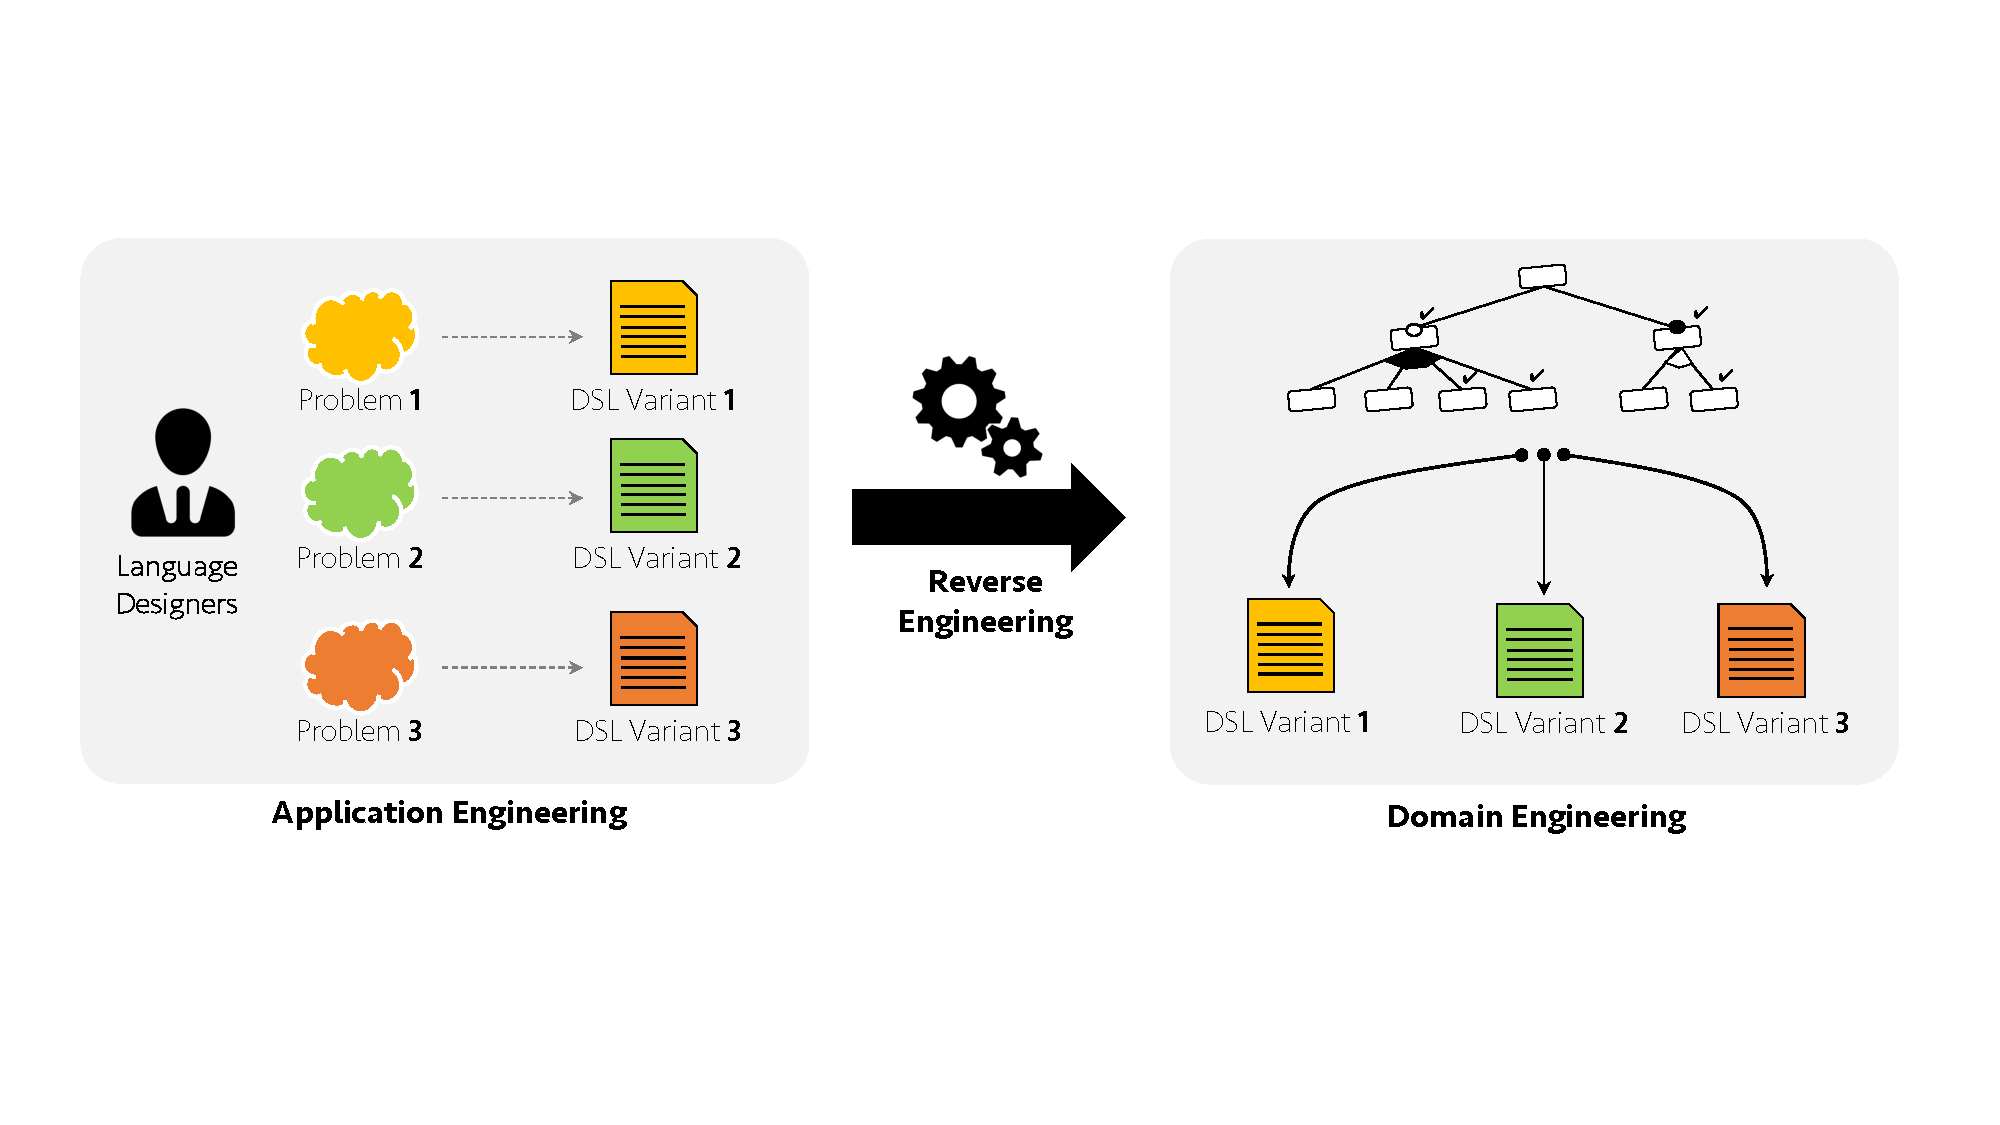
\includegraphics[width=0.8\linewidth]{images/bottom-up-lpl-fig.pdf}
%	\caption{Bottom-up language product lines engineering \label{fig:lple-dimensions}}
%\end{figure*}

%\vspace{2mm}
%\textit{\textbf{The clone-and-own approach.}} In this article, we are interested in bottom-up language product lines. Specifically, we propose a technique to reverse engineering language product lines from sets of existing DSL variants built through the \textit{clone-and-own} approach. With this approach, DSL variants are created by cloning existing versions of a DSL and performing certain adaptations intended to satisfy a specific purpose. While several research works have shown that the clone-and-own practice is common in software development projects \cite{Mayrand:1996,Rubin:2015}, in a recent work we provided empirical evidences that show that it is also a common practice during language development \cite{MendezAcuna:2016}. We conducted an analysis of a large pool of DSLs obtained from \texttt{GitHub}, and we detected a relevant amount of specification clones among them. You can found the sources of the experiments in a dedicated web-site\footnote{\url{http://empiricalpuzzle.weebly.com/}}.

%As a response to this phenomenon, recent research works have proposed mechanisms to reverse engineering software product lines from sets of existing software products which share code clones. This type of approaches are a clear example of bottom-up software product lines. and discussed its on software maintenance \cite{Chatterji:2016}

%Another important characteristic of the development process during the construction of bottom-up language product lines is that, in many cases, language designers use the copy/paste/modify pattern to create  individual DSLs. This approach is explained by Lopez Herrej\'on et all for the general case of software product lines.

\subsection{Motivating scenario} Suppose a team of language designers working on the construction of the DSL for finite state machines. Initially, language designers followed the UML specification \cite{UML:2011} to define language constructs such as states, regions, transitions, and triggers. Those language constructs are specified in terms of their syntax and semantics. So, at the end of the language development process, language designers release an executable DSL which behavior complies the UML specification.

Once this first DSL was released, the language designers are asked to build a new variant which must comply the Rhapsody specification \cite{Harel:2004} (i.e., another formalism to finite state machines). This new variant shares many commonalities with UML state machines, but introduces differences at both syntax and semantics levels \cite{Crane:2007}. After building this second variant, language designers obtained two different DSLs implementing different formalisms of state machines. Those DSL variants have some commonalities among them. And at the same time, the DSL have some particularities that make them unique.

Note that this process is repeated each time language designers have to build a new variant of the DSL for each new FSM formalism (e.g., Stateflow \cite{Martaj:2010} or Harel state machines \cite{Harel:1996}). This becomes specially challenging when final users need to combine some specifications to define hybrid formalisms. While several approaches have been proposed to reverse engineering software product lines from existing product variants \cite{LopezHerrejon:2015,Martinez:2015,Martinez:2015b}, in this article we propose techniques to reverse engineering language product lines from existing DSL variants.

\subsection{Scope: \textbf{Executable Domain Specific Languages}}
\label{sec:technologicalscope}

All the ideas presented in this article are focused to executable domain specific modeling languages (xDSMLs) where the abstract syntax is specified through \textit{metamodels}, and the dynamic semantics is specified operationally as a set of \textit{domain specific actions} \cite{Combemale:2013}. Whereas metamodels are class diagrams that represent language constructs and relationships among them, domain specific actions are Java-like methods that introduce behavior in the metaclasses of a given metamodel \cite{Jezequel:2015b}. 

Fig. \ref{fig:fig-dsl-example} illustrates this type of DSLs through a simple example on finite states machines. In that case, the metamodel that implements the abstract syntax contains three metaclasses: \textsl{StateMachine}, \textsl{State}, and \textsl{Transition}. There are some references among those metaclasses representing the relationships existing among the corresponding language constructs. The domain specific actions at the right of the Fig. \ref{fig:fig-dsl-example} introduce the operational semantics to the DSL. In this example, there is one domain specific action for each metaclass. Note that the interactions among domain specific actions can be internally specified in their implementation by means of the \textit{interpreter pattern}, or externalized in a model of computation \cite{Combemale:2013}.

\begin{figure}
\centering
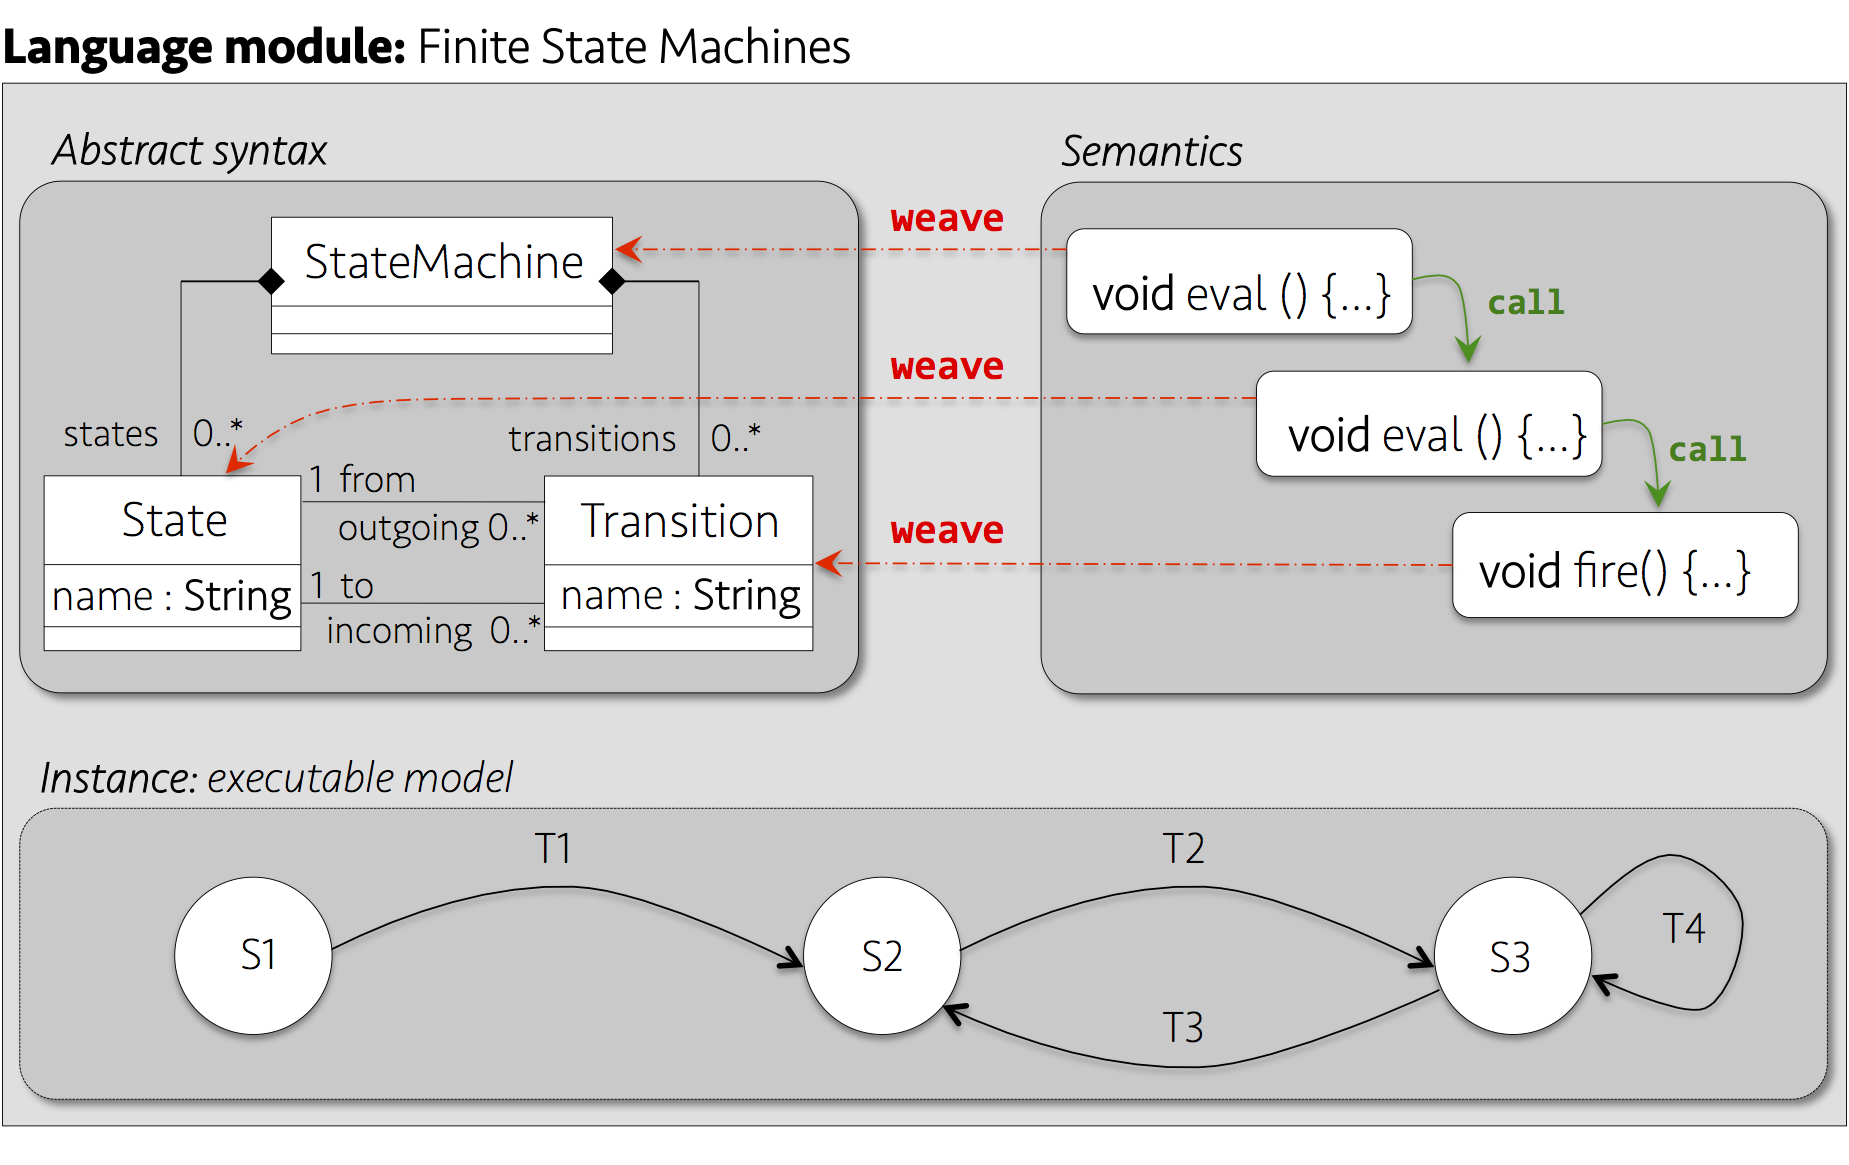
\includegraphics[width=1\linewidth]{images/fig-dsl-example.png}
\caption{A simple DSL for finite state machines}
\label{fig:fig-dsl-example}
\end{figure}

\section{Proposed Approach: \\ \textit{Reverse-Engineering Language Product Lines}}
\label{sec:approach}

In this section, we present our reverse engineering technique to support the construction of bottom-up language product lines. As shown in Fig. \ref{fig:reverse-engineering}, the proposed technique is composed of three steps. During the first step, we automatically recover a language modular design for the language product line. Such a modular design is composed of a set of language modules and a set of dependencies among them. During the second step, language modules' dependencies are used to synthesize a variability model that can be used, during the third step, to configure concrete DSL variants. Finally, during the forth step the DSL variant is assembled by composing the involved language modules. 

\begin{figure*}
\centering
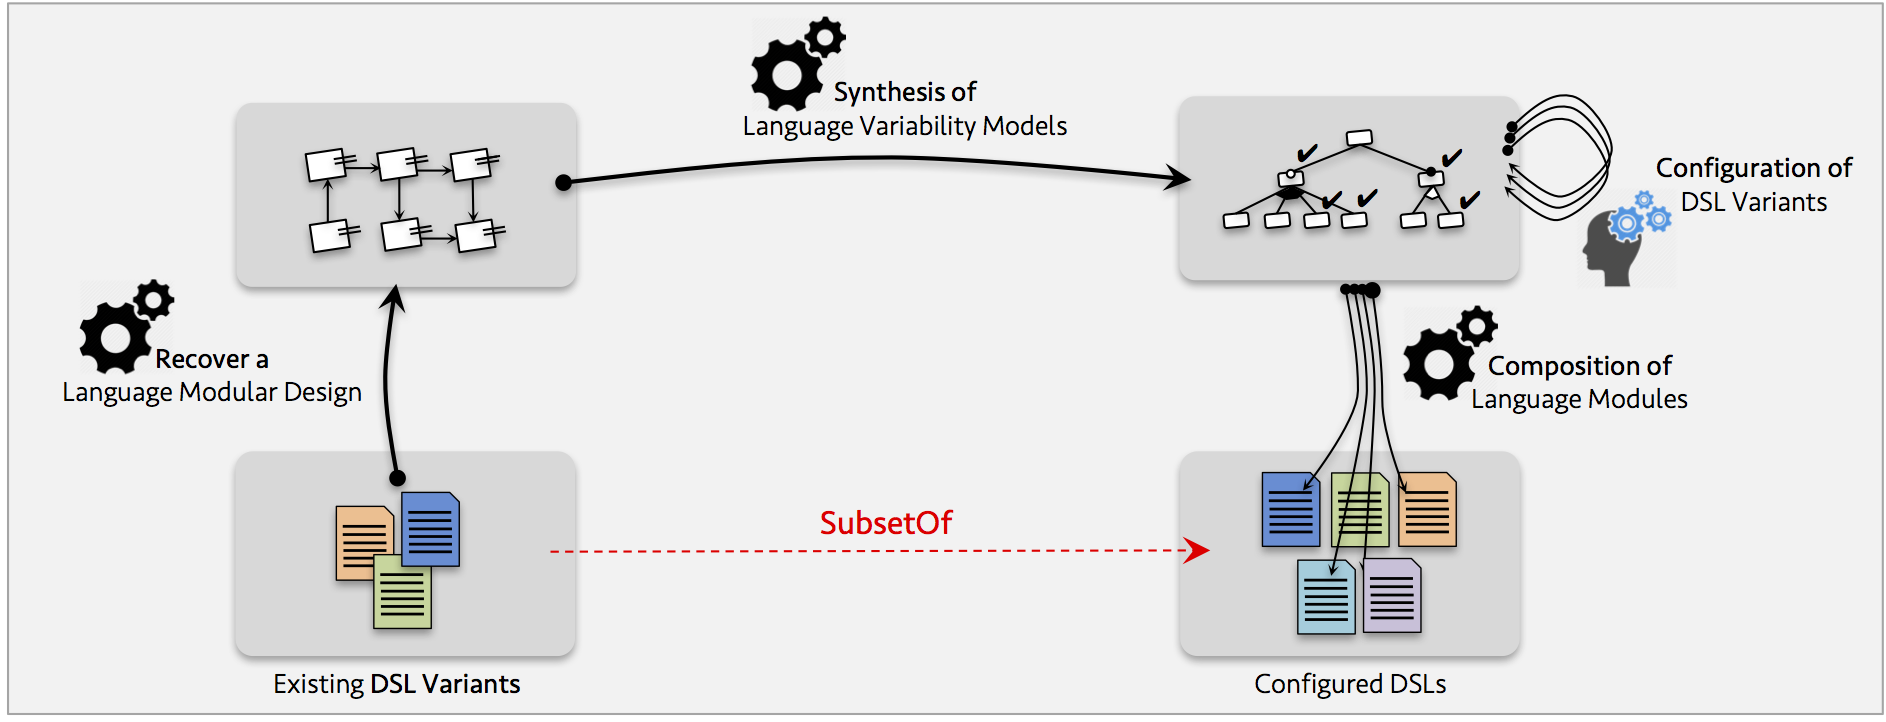
\includegraphics[width=1\linewidth]{images/reverse-engineering-overview.png}
\caption{Reverse engineering language product lines: approach overview}
\label{fig:reverse-engineering}
\end{figure*}

\subsection{Recovering a Language Modular Design}
\label{sec:reverseengineeringmodules}

Let us start the description of our reverse engineering technique by explaining the way in which we identify the set of language modules and dependencies that constitute the language modular design of the product line. The details of this recovering process are explained below as well as the way in which language modules are specified to guarantee their composability. 

\subsubsection{Language Modules. \textbf{How to identify them?}}

To identify the language modules of a language product line, we propose to take all the given DSL variants and unify them in a unique DSL. Then, the unified DSL is broken down into several interdependent language modules. This process results in a factorization of the specification clones existing in the DSL variants. The purpose of this strategy is to remove specification clones, thus reducing the maintenance costs. Such a factorization strategy is based on four principles explained in the following:

\vspace{2mm}
\emph{\textbf{Principle 1:} DSL specifications are comparable. So, specification clones can be automatically detected.} To detect the specification clones in a given set of DSL variants, we need to compare those specification clones and find out the repeated specification elements. For the technological space discussed in this article, specification elements for the abstract syntax correspond to metaclasses whereas specification elements for the semantics correspond to domain specific actions. Hence, comparison of DSL specifications corresponds to compare metaclasses and domain specific actions.

\vspace{2mm}
\emph{Comparison of metaclasses.} To compare metaclasses, we need to take into account that a metaclass is specified by a name, a set of attributes, and a set of references to other metaclasses. Two metaclasses are considered as equal (and so, they are clones) if all those elements match. Formally, comparison of metaclasses is formalized by the operator $\doteqdot$. %Comparing two metamodels relies on pair-wise comparison of all their metaclasses. 

\begin{equation}
  \doteqdot~: MC \times MC \rightarrow bool
\end{equation}
\begin{equation}
\begin{split}
  MC_{A} &\doteqdot MC_{B} = true \implies \\
   & MC_{A}.name = MC_{B}.name ~ \wedge \\
   & \forall a_1 \in MC_{A}.attr \mid (\exists a_2 \in MC_{B}.attr \mid a_1 = a_2) ~ \wedge \\
   & \forall r_1 \in MC_{A}.refs \mid (\exists r_2 \in MC_{B}.refs \mid r_1 = r_2) ~ \wedge \\
   & |MC_{A}.attr| = |MC_{B}.attr| ~ \wedge \\
   & |MC_{A}.refs| = |MC_{B}.refs|
  \end{split}
\end{equation}

\emph{Comparison of domain-specific actions.} To compare domain specific actions, we need to consider that --similarly to methods in Java-- domain specific actions have a signature that specifies its contract (i.e., return type, visibility, parameters, name, and so on), and a body where the behavior is implemented. Two domain specific actions are equal if their signatures and bodies are equivalent.

Whereas comparison of signatures can be performed by syntactic comparison of the signature elements, comparison of bodies can be arbitrary difficult. If we try to compare the behavior of the domain-specific actions, then we will have to address the semantic equivalence problem, which is known to be undecidable \cite{Lucanu:2013}. To address this issue, we conceive bodies comparison in terms of its abstract syntax tree as proposed by Biegel et al. \cite{Biegel:2010}. In other words, to compare two bodies, we first parse them to extract their abstract syntax tree, and then we compare those trees. Note that this decision makes sense because we are detecting specification clones more than equivalent behavior. Formally, comparison of domain-specific actions (DSAs) is specified by the operator $\fallingdotseq$.  

\begin{equation}
  \fallingdotseq~: DSA \times DSA \rightarrow bool
\end{equation}
\begin{equation}
\begin{split}
  DSA_{A} & \fallingdotseq DSA_{B} = true \implies \\
   & DSA_{A}.name = DSA_{B}.name ~ \wedge \\
   & DSA_{A}.returnType = DSA_{B}.returnType ~ \wedge \\
   & DSA_{A}.visibility = DSA_{B}.visibility ~ \wedge \\
   & \forall p_1 \in DSA_{A}.params \mid \\
   & (\exists p_2 \in DSA_{B}.params \mid p_1 = p_2)  ~ \wedge \\
   & |DSA_{A}.params| = |DSA_{B}.params|  ~ \wedge \\
   & DSA_{A}.AST = DSA_{B}.AST
 \end{split}
\end{equation}

\vspace{2mm}
\emph{\textbf{Principle 2:} Specification clones can be viewed as sets' intersections, which is useful to factorization.} A DSL specification can be seen as a set of metaclasses and a set of domain specific actions. In doing so, specification clones correspond to intersections among those sets. Those intersection elements can be specified once and reused in several DSL variants \cite[p. 60-61]{Voelter:2013b}. Hence, we can factorize specification clones by breaking down the intersections existing among DSL specifications.

Fig. \ref{fig:shape} illustrates this observation through the running example introduced in Section \ref{sec:problemstatement}. At the left of the figure, we show two Venn diagrams to represent both syntax and semantic intersections. The Venn diagram corresponding to the abstract syntax shows that the classical constructs for state machines such as StateMachine, State, and Transition are in the intersection of the three given DSL variants i.e., UML state machines, Rhapsody, and Harel's state machines. In turn, there are certain particularities for each DSL. For example, the concept AndTrigger is owned by UML and Harel state machines but not for Rhapsody. Concepts such as OrTrigger and NotTrigger are only provided by Harel state machines since the concept of Choice is exclusive of UML state machines.

For the case of semantic variability, the 3-sets intersection is empty. It means that there is not a common semantic for the three DSL variants. Rather, UML state machines and Rhapsody share the domain specific actions corresponding to the constructs of State Machine, State, and Transition. In turn, the implementation of Harel state machines is different. 

This way to conceive DSL specifications is useful to factorize specification clones as illustrated at the right of the Fig. \ref{fig:shape}. Each different intersection is separated in a separate subset that, as we will explain later, is encapsulated in a language module. 

\begin{figure*}
\centering
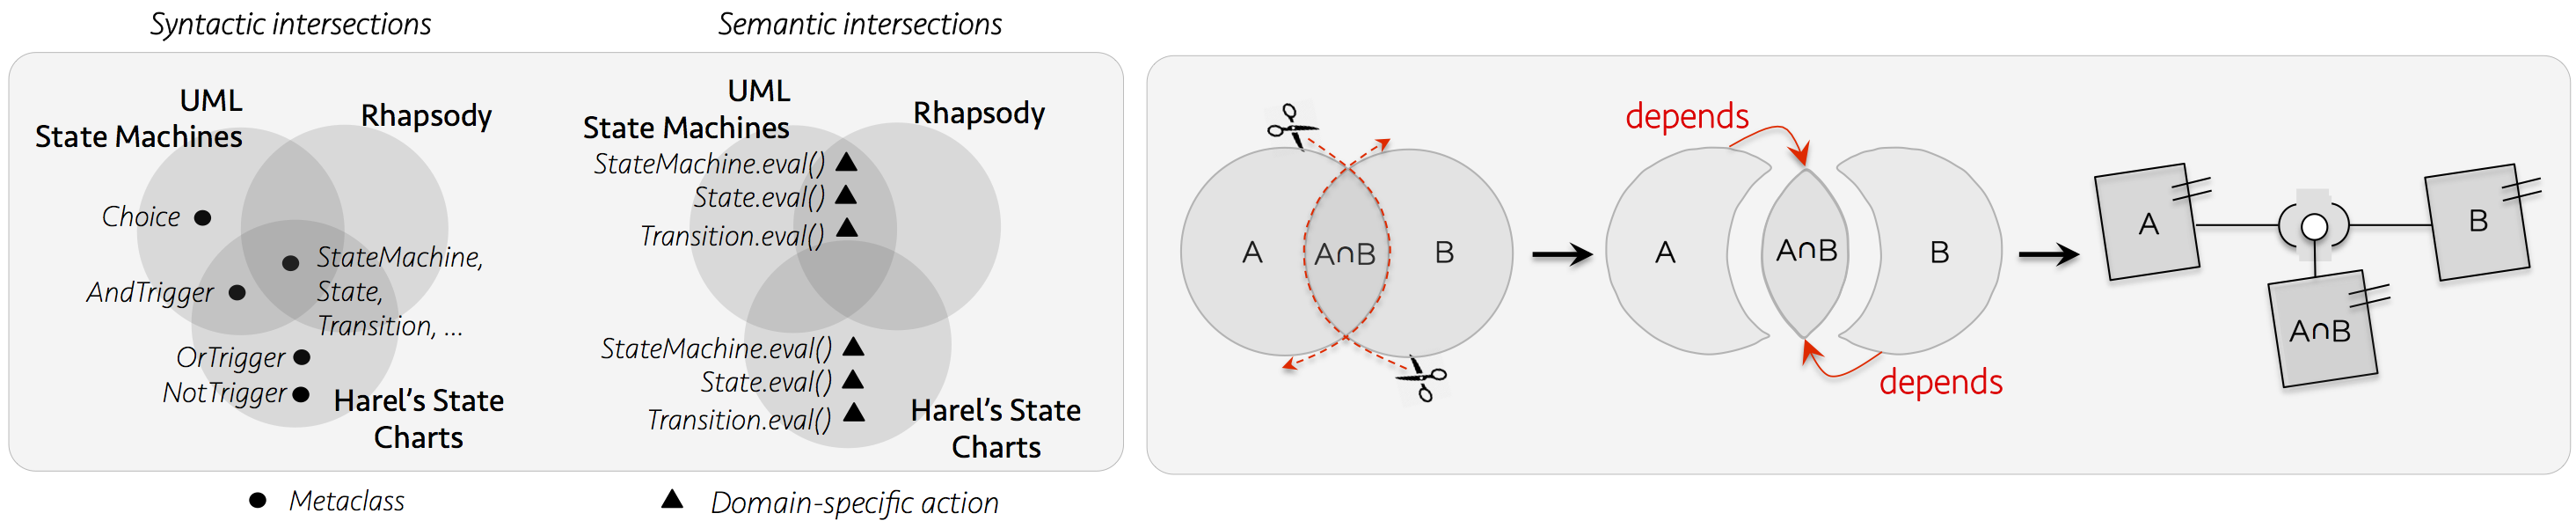
\includegraphics[width=1\linewidth]{images/principle2.png}
\caption{Factorizing specification clones from DSL variants}
\label{fig:shape}
\end{figure*}

%\vspace{2mm}
%\textit{\textbf{Principle 3:} Breaking down overlapping is useful to factorize specification clones.} According to principle 2, overlapping between two DSLs implies the existence of repeated metaclasses and/or domain specific actions i.e., specification clones. Those repeated elements can be specified once and reused in the two DSLs \cite[p. 60-61]{Voelter:2013b}. Hence, we can factorize specification clones by breaking down the overlapping existing among DSL specifications as illustrated in Figure \ref{fig:cutting}; 

%\begin{figure}
%\centering
%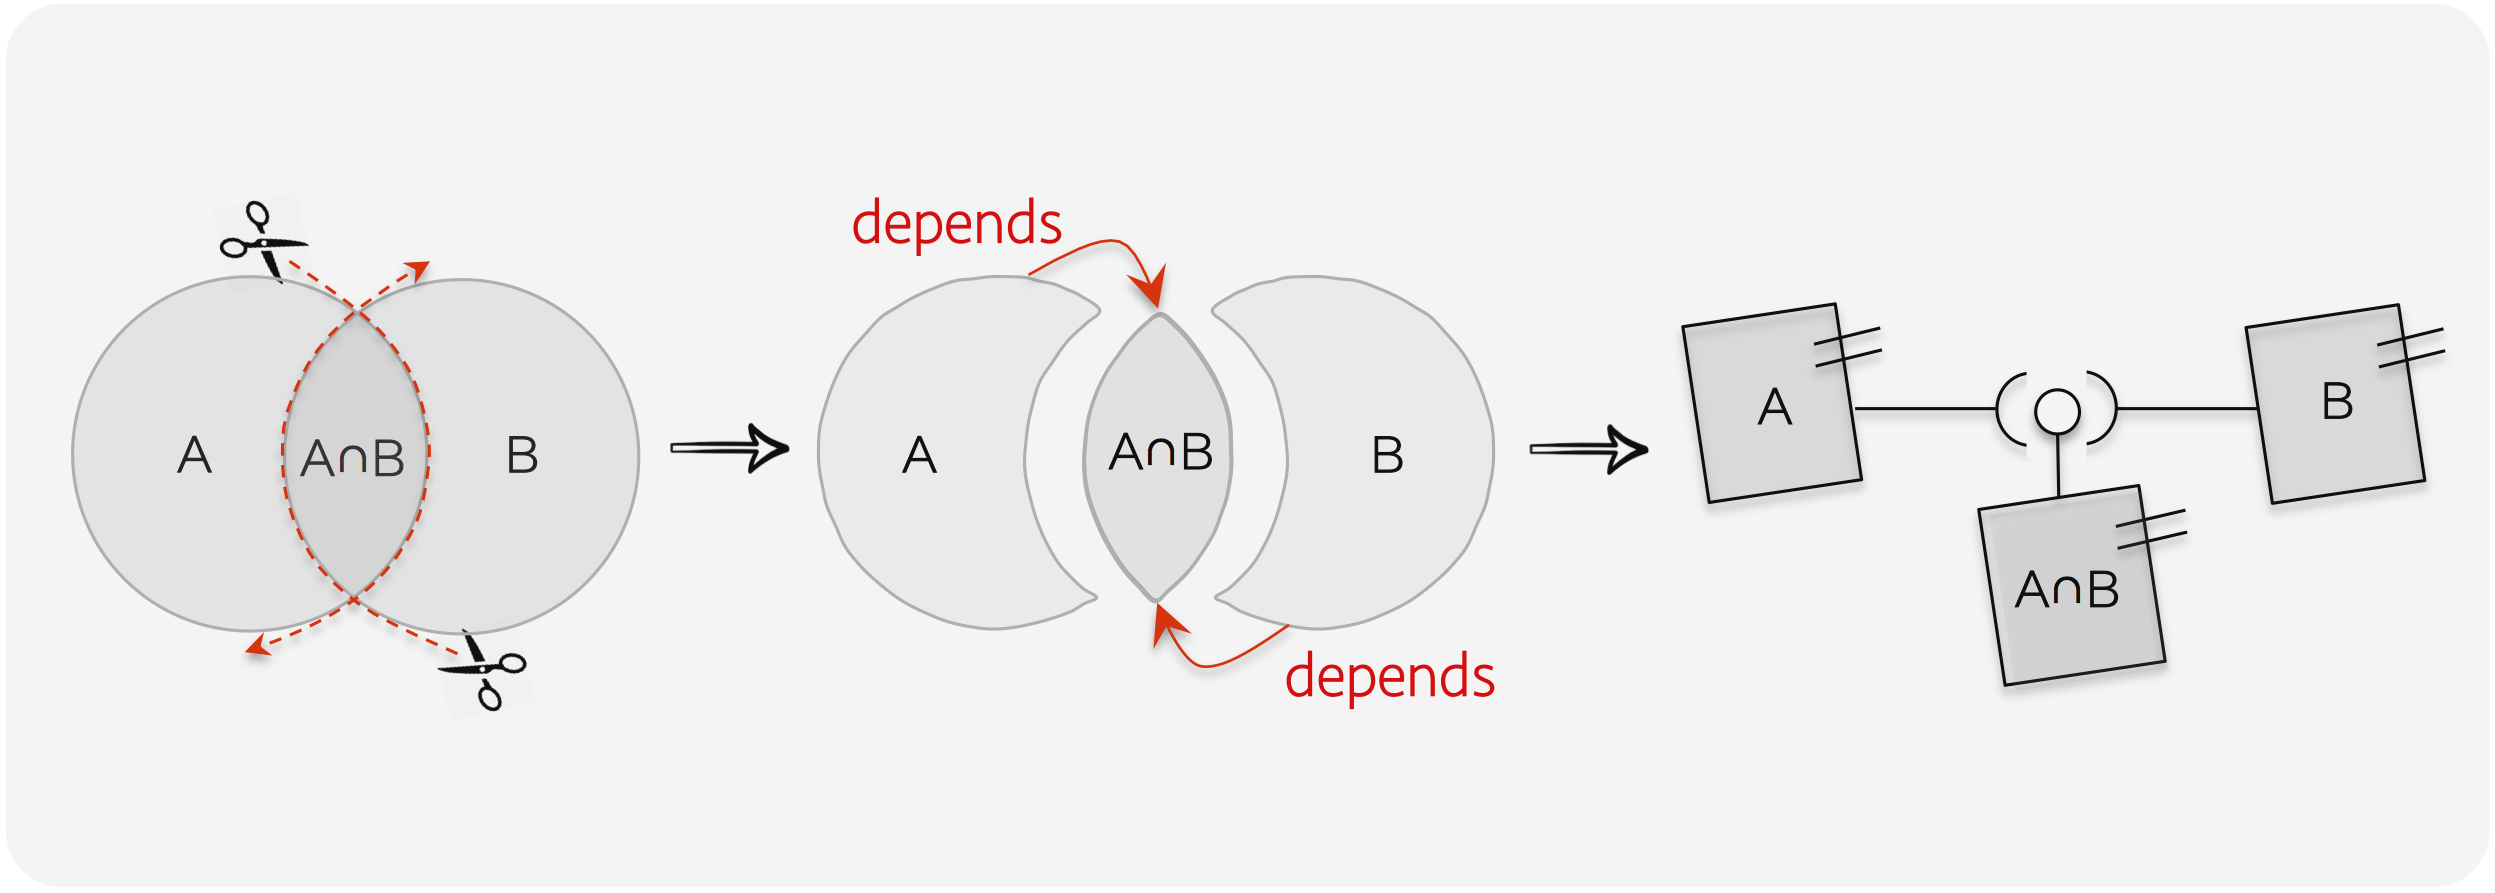
\includegraphics[width=0.97\linewidth]{images/fig-breaking-overlapping.png}
%\caption{Breaking down overlapping to obtain language modules}
%\label{fig:cutting}
%\end{figure}

\vspace{2mm}
\textit{\textbf{Principle 3:} Abstract syntax first, semantics afterwards.} The abstract syntax is the backbone of the DSL specification; it specifies its structure in terms of metaclasses and relationships among them whereas the domain-specific actions add executability to the metaclasses. Hence, the process of breaking down intersections should be performed for the abstract syntax first, thus identifying the way in which metaclasses should be grouped into the different language modules. Afterwards, we can do the proper for the semantics. In doing so, we need to take into consideration the phenomenon of semantic variability. That is, two cloned metaclasses might have different domain-specific actions. That occurs when two DSLs share some syntax specification but differ in their semantics.

\vspace{2mm}
\textit{\textbf{Principle 4:} Breaking down a metamodel is a graph partitioning problem.} A metamodel can be seen as a directed graph $G=<V,A>$ where:

\begin{itemize}
\item \textbf{V}: is the set of vertices each of which represents a metaclass.
\item \textbf{A}: is the set of arcs each of which represents a relationship between two metaclasses i.e., references, containments, and inheritances.
\end{itemize}

This observation is useful for breaking down metamodels, which can be viewed as a graph partitioning problem where the result is a finite set of subgraphs. Each subgraph represents the metamodel of a reusable language module.

\vspace{2mm}
\textbf{\textit{The principles in action.}} Fig. \ref{fig:breakingdown} shows the way in which we recover a language modular design through the principles explained above. It is composed of two steps: unification and breaking down.

\begin{figure*}
\centering
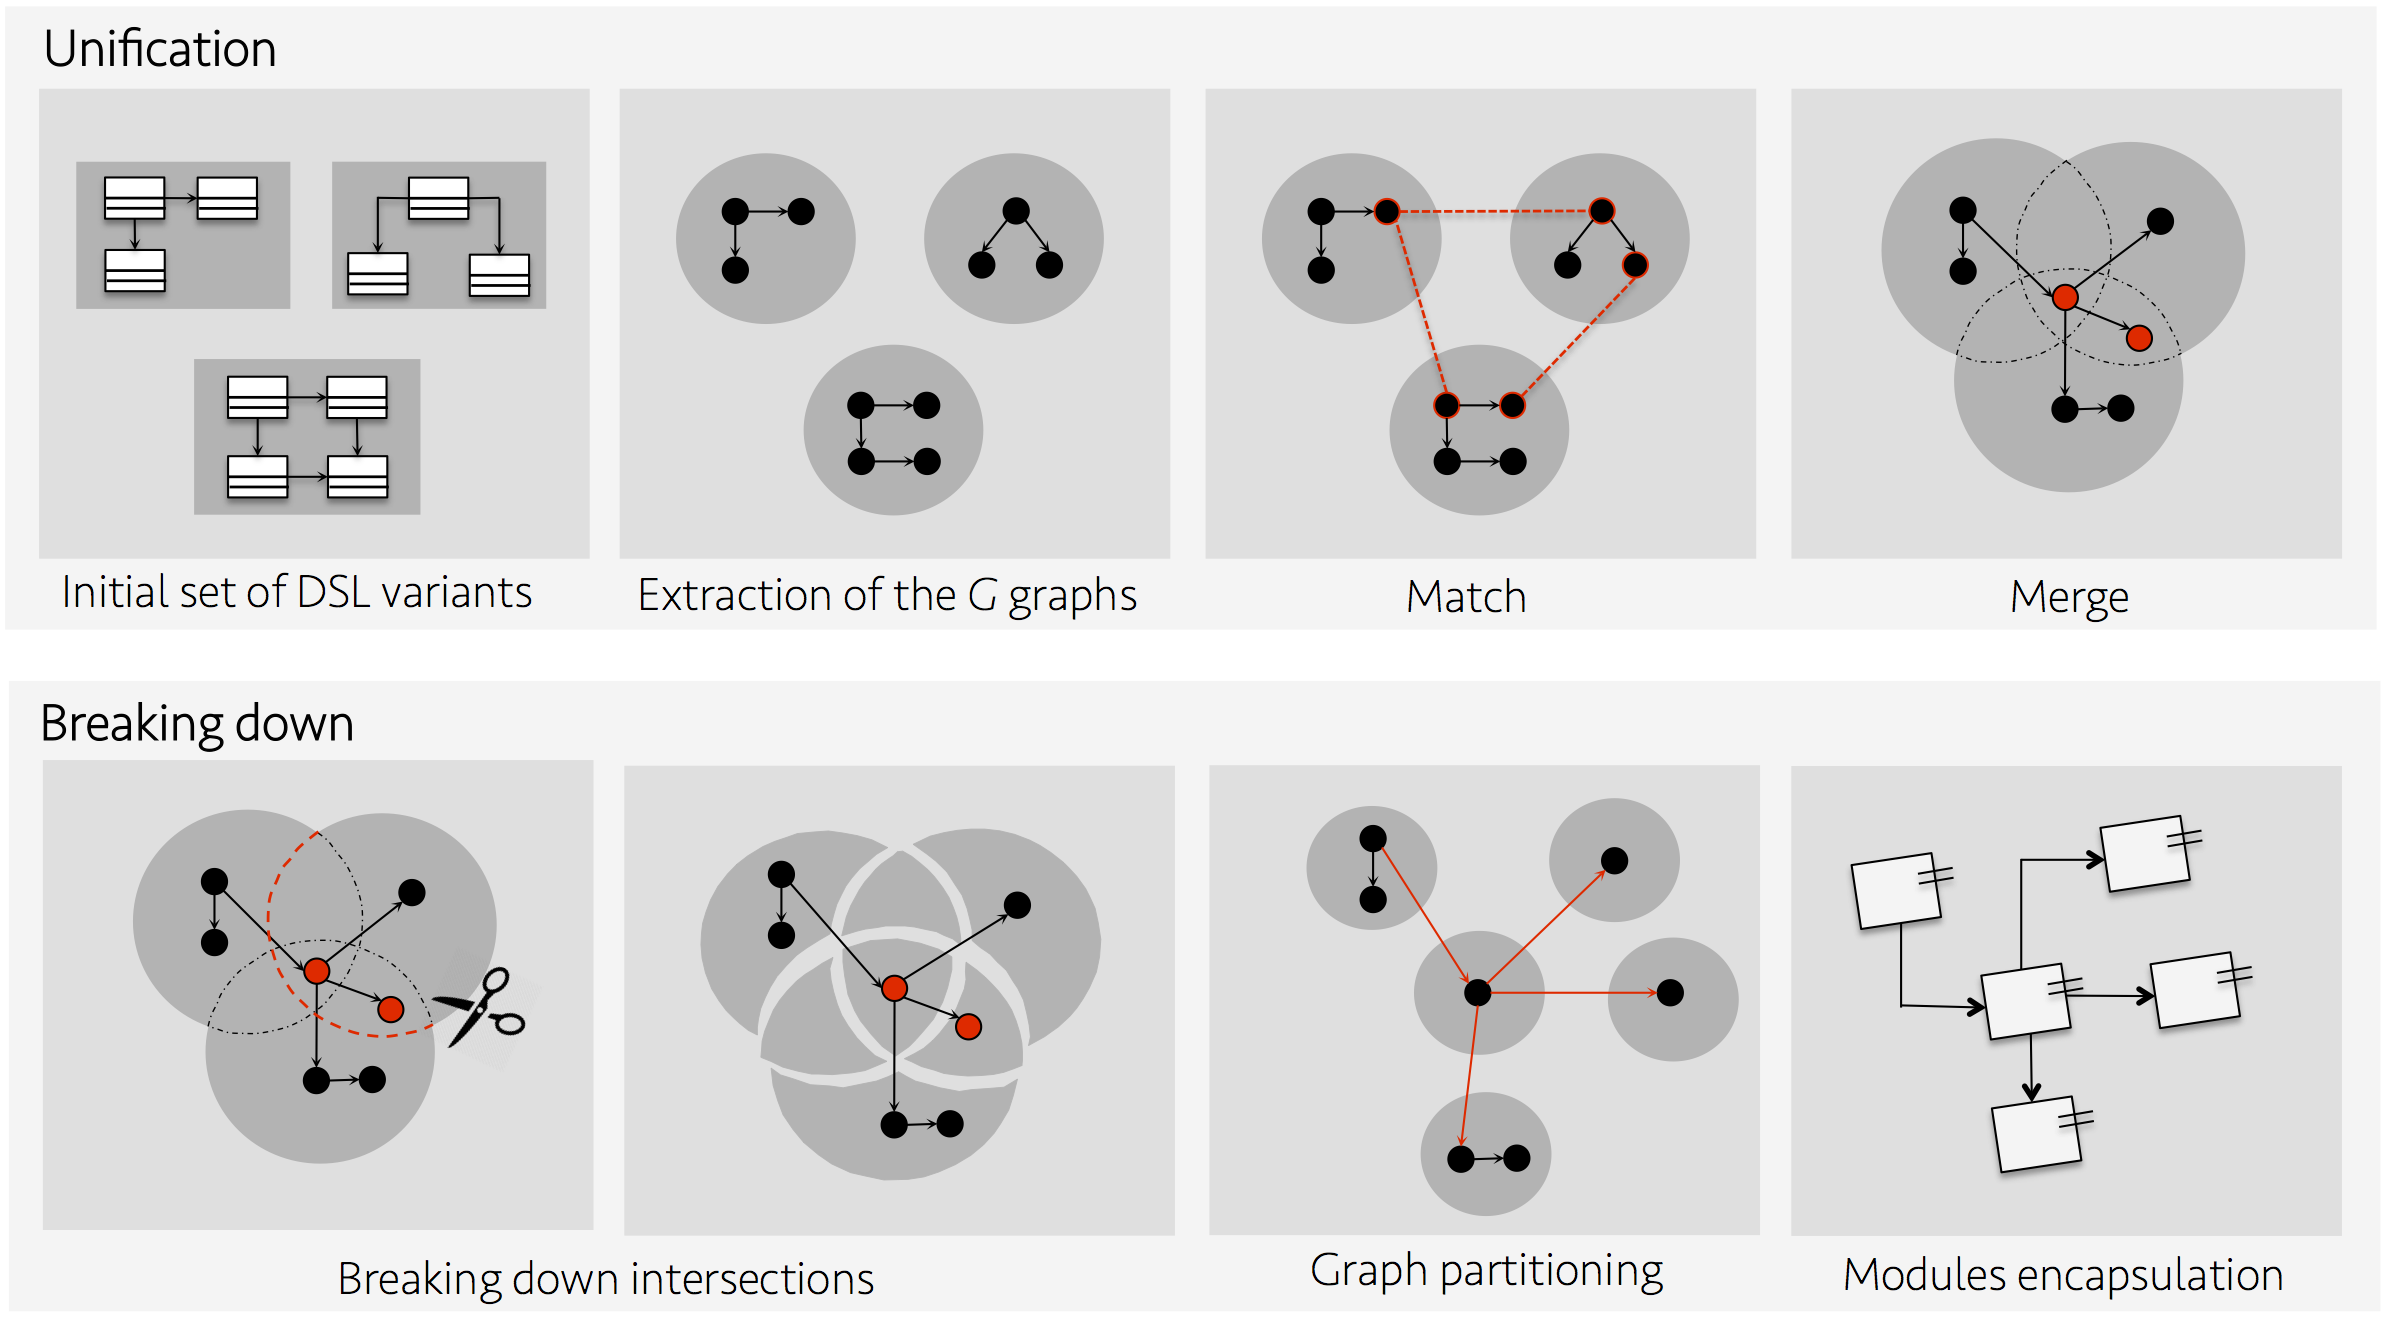
\includegraphics[width=1\linewidth]{images/fig-reverse-engineering-detailed.png}
\caption{Unifying and breaking down for recovering a language modular design}
\label{fig:breakingdown}
\end{figure*}

\vspace{2mm}
\textit{Unification: \textbf{match} and \textbf{merge}.} The objective of this step is to unify all the DSL variants in a unique specification. To this end, we first produce a graph $G$ for the metamodel of each DSL variant according to the principle 4. Second, we use the comparison operators defined in the principle 1 to match the vertices representing the metaclasses repeated in two or more DSL variants. Third, we create the syntactic intersections defined in principle 2 by merging the matched vertices. In doing so, we remove cloned metaclasses. After this process, we have a unified graph (which is not necessarily a connected graph) including all the metaclasses provided in the DSL variants. 

To identify semantic intersections, we check whether the domain specific actions of the matched metaclasses are equal. If so, they can be considered as semantic specification clones, and they are also merged. If not all the domain specific actions associated to the matched metaclasses are equal, different clusters of domain specific actions are created, thus establishing semantic variation points.

\vspace{2mm}
\textit{Breaking down: \textbf{cut} and \textbf{encapsulate}.} Once intersections among the DSL variants have been identified, we factorize the specification clones. To this end, we break down the unified graph using a graph partitioning algorithm. Our algorithm returns a set of clusters of vertices: one cluster for each intersection of the Venn diagram. Arcs defined between vertices in different clusters can be considered as cross-cutting dependencies between clusters. Finally, we encapsulate each vertex cluster in the form of a language module. 

\subsubsection{Language Modules. \textbf{How to specify them?}}

We have explained the way in which we recover a language modular design by identifying clusters of language constructs and dependencies among them. However, it is unclear how to specify those clusters in concrete implementation artifacts that can be later composed. To answer deal with this issue, we propose to specify a language module in terms of (1) a metamodel containing the metaclasses corresponding to each construct cluster; and (2) a set of domain specific actions implementing the semantics of their metaclasses (see Fig. \ref{fig:modulespec}). If there is semantic variability, then a language module can have several clusters of domain specific actions. The dependencies among language modules are materialized through required and provided interfaces. 

\begin{figure}[h!]
\centering
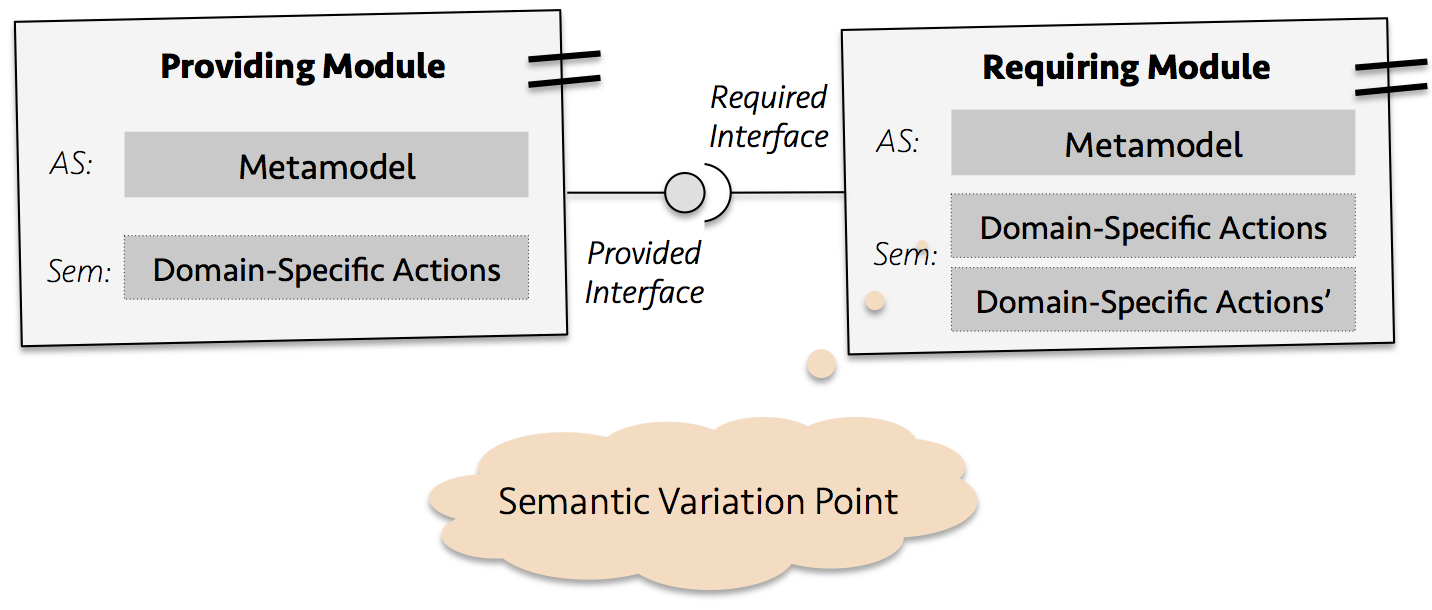
\includegraphics[width=1\linewidth]{images/language-modules-specification.png}
\caption{Specification of language modules}
\label{fig:modulespec}
\end{figure}



\vspace{2mm}
\textit{\textbf{Required interfaces.}} A required interface is a mechanism to declare the needs that a language module has towards other modules while assuming that their needs will be eventually fulfilled. Suppose for example the development of a language module for finite state machines. This language module needs some additional abstractions such as constraints to express guards in the transitions. Using a required interface, those needs can be declared as a set of required constructs (e.g., \textsl{Constraint}). 

We propose a mechanism to distinguish whether a given language specification element (i.e., meta-class, property, operation, parameter, enumeration, etc) corresponds to an actual implementation or a required declaration. The proposed mechanism is an extension to the EMOF meta-language that introduces the notion of ``requirement", so we can define \textit{required specification elements} in metamodels. When encapsulating clusters of concepts in language modules, all the constructs contained in the cluster are defined as actual implementations. In turn, all the references to specification elements that belong to other clusters are defined as required specification elements, so they are included in the required interface. 

%

%Fig. \ref{fig:fig-req-example-fig} illustrates the use of required interfaces through the example introduced before regarding a language module for finite state machines that requires a constraint language. In that example, the constructs proper the state machines are non-virtual elements since they correspond to actual implementation of such abstractions. In turn, the constraints to express the guards in the transitions are expressed as a virtual construct called \textsl{Constraint} that provides a virtual operation action called \textsl{eval()} which is used in the specification of the semantics of the meta-class \textsl{Transition}. 

%\begin{figure}
%  \centering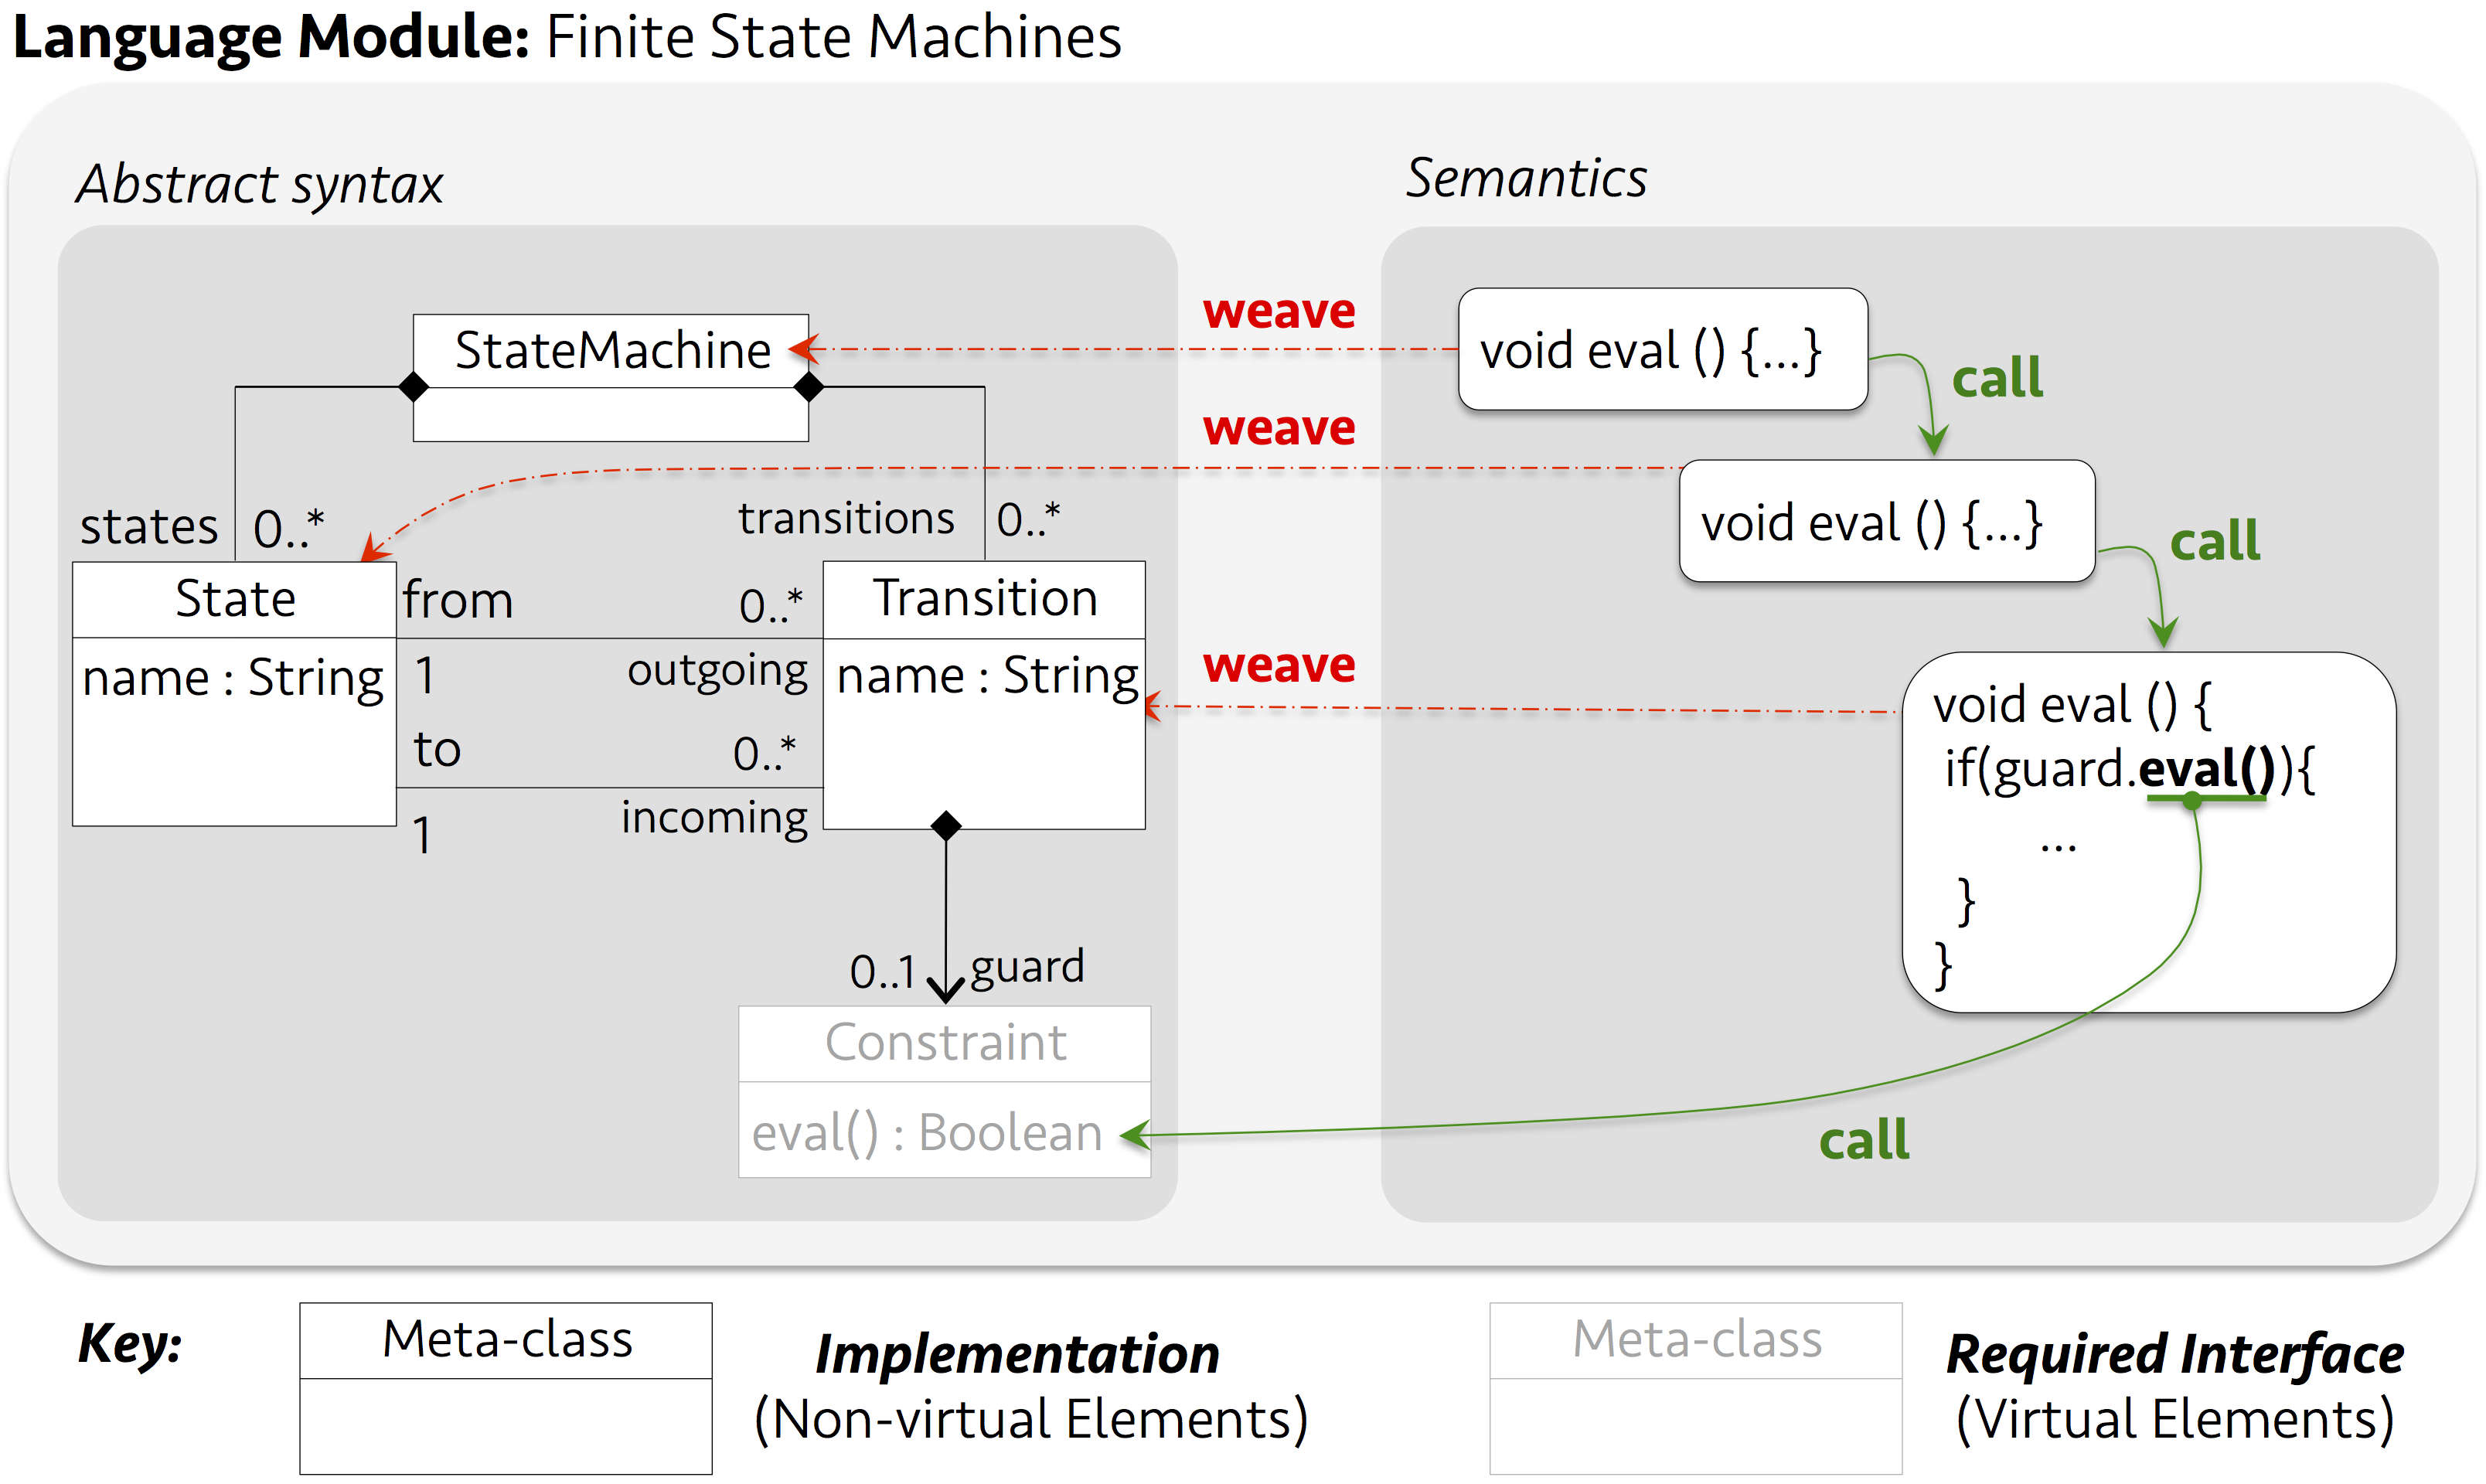
\includegraphics[width=0.86\linewidth]{images/fig-req-example-fig.png}
%  \caption{Example of the use of required interfaces}
%  \label{fig:fig-req-example-fig} 
%\end{figure}

\vspace{2mm}
\textit{\textbf{Provided interfaces.}} The purpose of provided interfaces is to expose the functionality offered by the language module. Consider for example a language module that offers the capability to express and evaluate constraints. Using a providing interface, language designers can express the essential functionality of the module i.e., expression and evaluation of constraints; and hide the implementation details and auxiliary concepts needed to achieve such functionality e.g., context management.

To support the definition of provided interfaces, we propose to extend EMOF with the notion of \textit{module visibility}. This extension allows to classify a certain specification element as either \textsl{\textbf{public}} or \textsl{\textbf{private}} according to its nature. For example, a language designer can classify a meta-class as \textsl{\textbf{public}} meaning that it represents essential functionality of the module so can be used by external modules and it belongs to the provided interface. Naturally, if the meta-class is classified as \textsl{\textbf{private}} it cannot be used by external modules and it cannot be considered as part of the provided interface. Note that the notion of module visibility is different from the notion of visibility already defined in EMOF. The later is associated to  certain access constraints of model elements with respect to the package in which they are implemented.

When encapsulating a language module from a cluster of constructs, all the constructs that are used by external clusters are defined as public.

%Fig. \ref{fig:fig-prov-example-fig} illustrates the use of provided interfaces through the example regarding the constraints module. Since the main functionality of the module is to define and evaluate constraints, the meta-classes included in the provided interface (so those one defined as \textsl{\textbf{public}} in terms of module visibility) are: \textsl{ConstrainedProgram} and \textsl{Constraint} including the operations that implement their semantics.

%\begin{figure}
%  \centering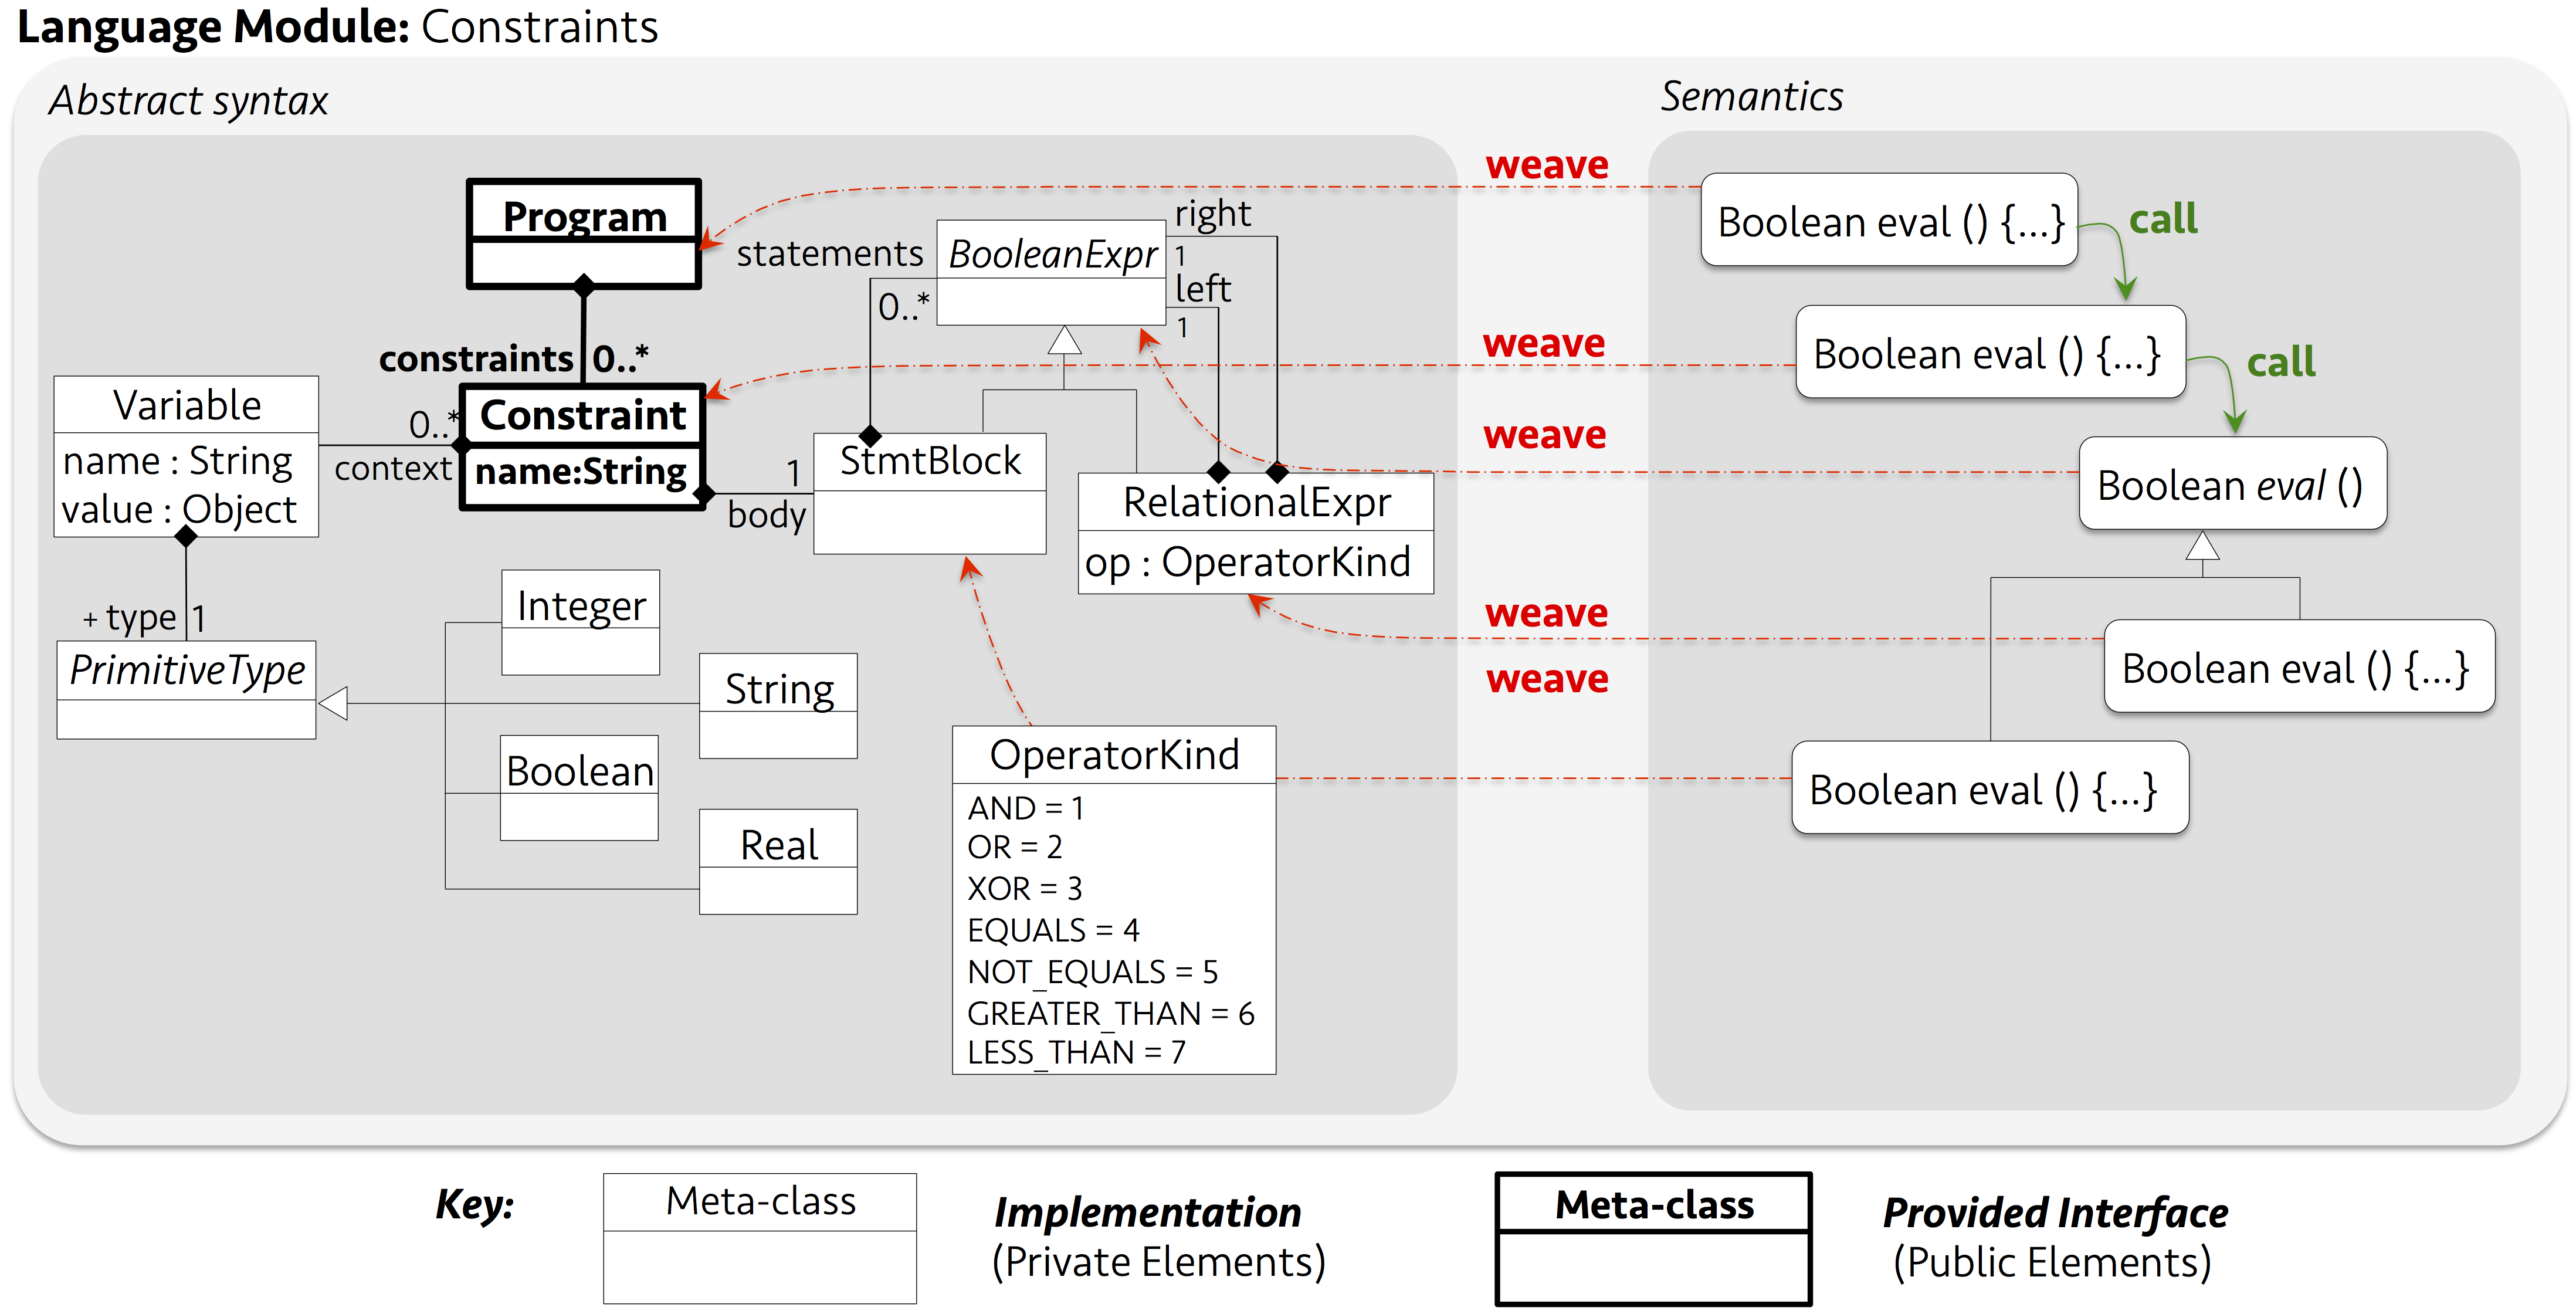
\includegraphics[width=1\linewidth]{images/fig-prov-example-fig.png}
%  \caption{Example of the use of provided interfaces}
%  \label{fig:fig-prov-example-fig}
%\end{figure}

\subsection{Synthesizing Language Variability Models}

Once we have recovered a language modular design for the language product line, we need to represent the existing variability in a model that permits to configure concrete DSLs. To this end, we need to find out an appropriated formalism for express that model, and then to conceive a strategy to synthesize those models from the language modular design. 

\subsubsection{Language Variability. \textbf{How to express it?}}

The challenge towards representing the variability existing in a language product line is that such variability is multi dimensional. Because the specification of a DSL involves several implementation concerns\footnote{Just as traditional general purpose languages, domain specific languages are typically defined through three implementation concerns: abstract syntax, concrete syntax, and semantics \cite{Harel:2004b}.}, then there are several dimensions of variability that we must manage: abstract syntax variability, concrete syntax variability, and semantic variability \cite{Cengarle:2009,Gronniger:2011}.

Abstract syntax variability refers to the capability of selecting the desired language constructs for a particular type of user. Concrete syntax variability refers to the capability of supporting different representations for the same language construct. Finally, semantic variability refers to the capability of supporting different interpretations for the same language construct. As the same as our approach to language modularization, our approach to variability management is scoped to abstract syntax and semantics; concrete syntax --and hence, concrete syntax variability-- is not being considered in the solution. 

%In this section we present a strategy to deal with this type of variability. To this end, we present an approach to represent the variability existing in a language product line. Then, we explain how we can use the variability models to configure concrete DSLs. As the same as our approach to language modularization, our approach to variability management is scoped to abstract syntax and semantics; concrete syntax --and hence, concrete syntax variability-- is not being considered in the solution. 

\vspace{2mm}
\textbf{\textit{Modeling multi-dimensional variability.}} A solution to represent abstract syntax variability and semantic variability should consider two main issues. Firstly, the definition of the semantics has a strong dependency to the definition of the abstract syntax --the domain-specific actions that implement the semantics of a DSL are weaved in the meta-classes defined in the abstract syntax--. Hence, these dimensions of variability are not isolated each other. Rather, the decisions made in the configuration of the abstract syntax variability impact the decisions that can be made in the configuration of the semantic variability. 

The second issue to consider at the moment of dealing with language variability management is that a semantic variation point might be transversal to several meta-classes. Moreover, if the involve meta-classes are introduced by different language modules in the abstract syntax, then the semantic variation point depends of two features. As a result, the relationship between a feature in the abstract syntax and a semantic variation point is not necessarily one-to-one. 

%For example, there is a semantic variation point in hierarchical state machines that corresponds to decide if the state machine follows either the run-to-completion policy or if it supports simultaneous events \cite{Crane:2007}. In any case, the implementation of this semantics involves code in domain-specific actions for the \textsl{StateMachine} and \textsl{Region} meta-classes. 

Currently, we can find several approaches to support multi dimensional variability (e.g., \cite{Rosenmuller:2011}). Some of those approaches have been applied concretely to language product lines \cite{Liebig:2013}. The most common practice is to use feature models to represent all the dimensions of variability. Each dimension is specified in a different tree and dependencies among decisions in those dimensions are expressed as cross-tree constraints. In this article, we propose a different approach based on the combination of feature models with orthogonal variability models. Feature models are used to model abstract syntax variability and orthogonal variability models are used to model semantic variability.

Fig. \ref{fig:languages-variability-modeling} illustrates our approach. At the top of the figure, there is a feature model in which each feature represents a language module. As aforementioned, each language module is composed of a metamodel and a set of domain specific actions. Hence, such a feature model is enough for language product lines where there is not semantic variability i.e., each language module has only one set of domain specific actions. Differently, when there are one or more language modules containing several sets of domain specific actions, then we have semantic variability that must be represented in the variability model. To represent such a variability, we include an orthogonal variability model as illustrated at the bottom of Fig. \ref{fig:languages-variability-modeling} which contains a variation point for each feature that represents a language module with more than one set of domain specific actions.

\begin{figure*}
  \centering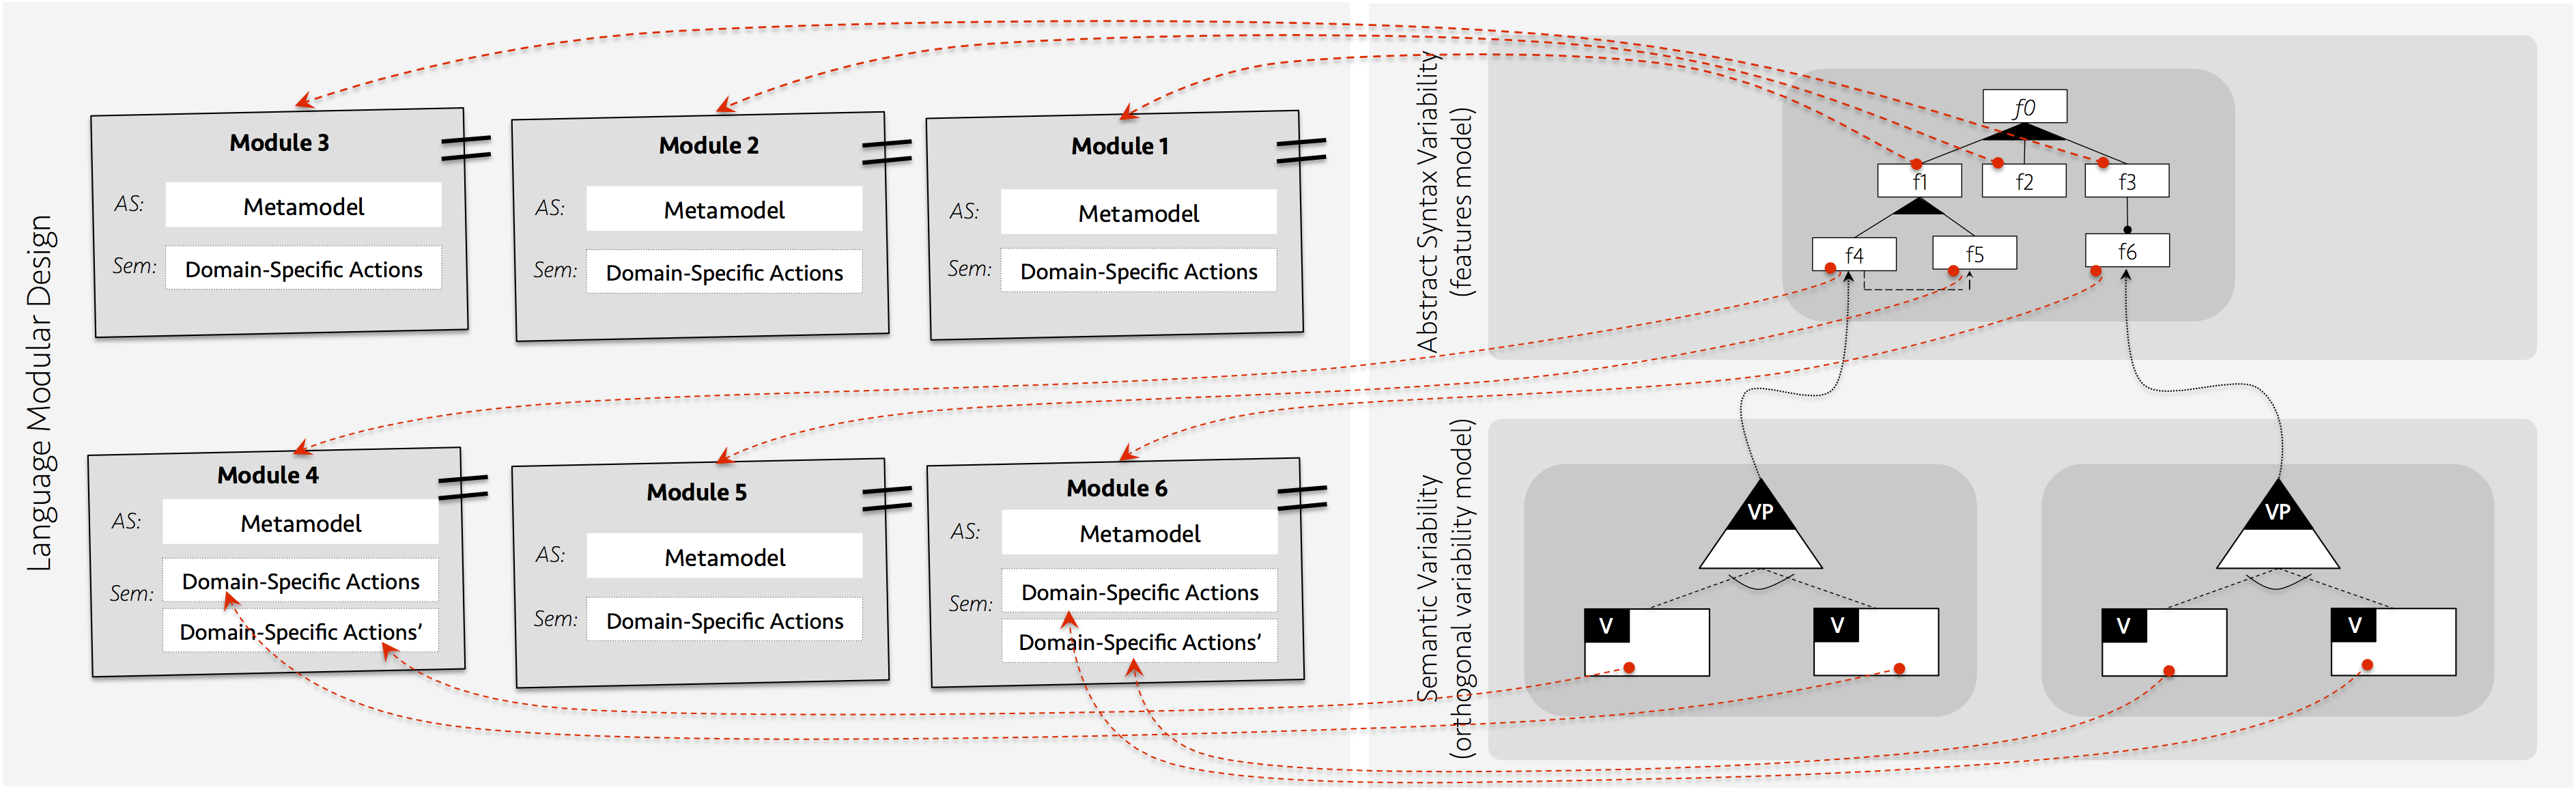
\includegraphics[width=1\linewidth]{images/language-variability-fig.png}
  \caption{Approach to represent multi-dimensional variability in language product lines}
  \label{fig:languages-variability-modeling}
\end{figure*}

\vspace{2mm}
\textit{\textbf{Why orthogonal variability models?}} An inevitable question that we need to answer at this point is: why we use orthogonal variability models instead of using feature models as proposed by current approaches? The answer to this questions is three-fold:

\vspace{2mm}
\textit{(1) The structure of orthogonal variability models is more appropriated.} As explained by Roos-Frantz et al. \cite{Roos-Frantz:2012}, feature models and orthogonal variability models are similar. However, they have some structural differences. One of those differences is that whereas a feature model is a tree that can have many levels, an orthogonal variability model is a set of trees each of which has two levels. Each tree represent one variability point and its children represent variants to that variation point. 

Semantic variation points are decisions with respect to a particular segment of the semantics of a language. Although those decisions can have some dependencies among them, they can hardly be organized in a hierarchy. Indeed, we conducted an experiment where we use feature models to represent semantic variation points, and we always obtained two-level trees: the first level corresponds to the name of the variation point and its children represent the possible decisions. This fact suggests that orthogonal variability models are more appropriated than feature models to represent semantic variability.  

\vspace{2mm}
\textit{(2) The meaning of orthogonal variability models is more appropriated.} According to \cite{Liebig:2013}, a language feature is a characteristic provided by the language which is visible to the final user. This definition can be associated abstract syntax variability and the use of feature models can be appropriated to represented it. All the approaches on language product line engineering use feature models to this end showing that it is possible and appropriated. 

The case of the semantic variability is different. A semantic decision is not a characteristic of a language that we can select or discard. The semantic of a DSL should be always specified if the DSLs is intended to be executable. Rather, a semantic decision is more a variation point that can have different interpretations captured as variants. This vocabulary fits better in the definitions provided by orthogonal variability models. More than features, we have variation points and variants, which also suggest that the use orthogonal variability models is more appropriate to represent semantic variability.

\subsubsection{Language Variability. \textbf{How to synthesize it?}}

Once we established an approach to represent language variability, we define an algorithm to synthesize variability models from a given language modular design. This algorithm produces not only a feature model with the abstract syntax variability, but also an orthogonal variability model representing the semantic variability. An overview of the approach is presented in Fig. \ref{fig:everse-engineering-vm}. 

\begin{figure*}
\centering
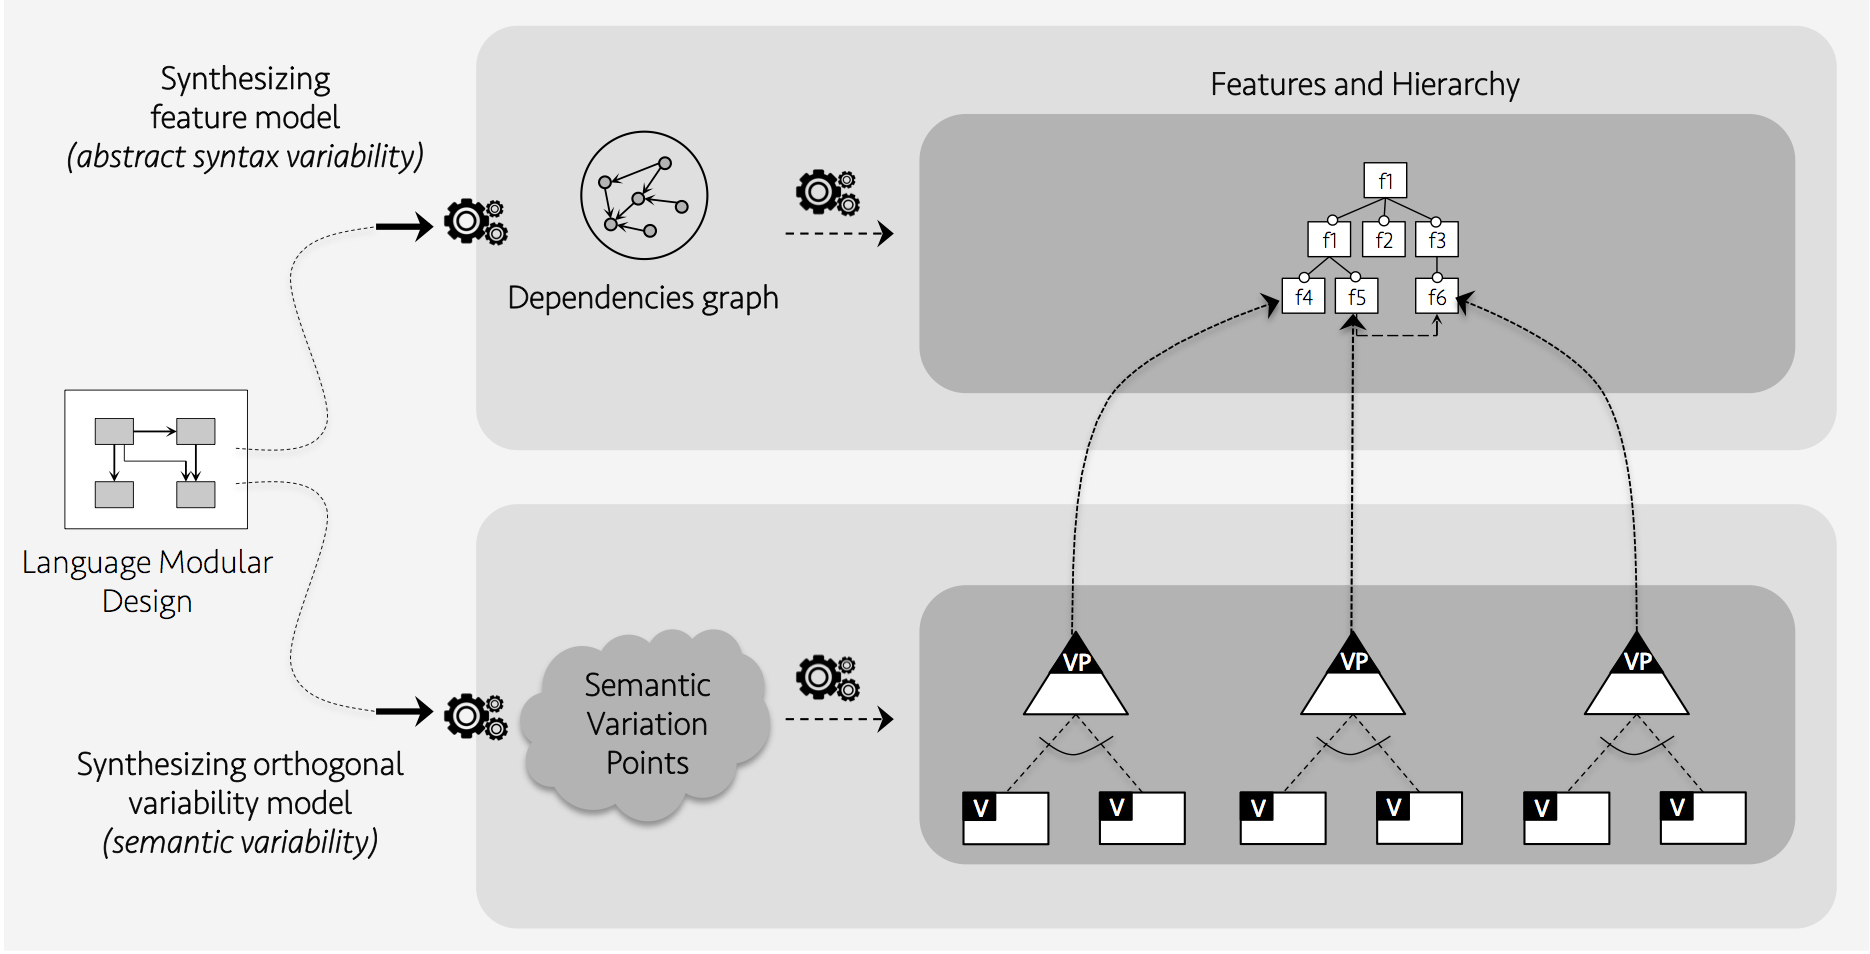
\includegraphics[width=1\linewidth]{images/reverse-engineering-vm.png}
\caption{Reverse-engineering variability models for language product lines}
\label{fig:everse-engineering-vm}
\end{figure*}

\vspace{2mm}
\textit{\textbf{Synthesizing abstract syntax variability.}} The first step to represent the variability of a language product line is to extract the feature model that represents the abstract syntax variability. To this end, we need an algorithm that receives the dependencies graph between the language modules, and produces a feature model which includes a set of features representing the given language modules as well as a set of constraints representing the dependencies among those modules. The produced feature model must guarantee that all the valid configurations (i.e., those that respect the constraints) produce correct DSLs.

In the literature, there are several approaches for reverse engineering feature modules from dependencies graphs (consider for example the approach presented by Assun\c{c}ao et al. \cite{Assuncao:2015}, or the one presented by She et al., \cite{She:2014}). In our case, we opt for an algorithm that produces a simple feature model where each language module is represented in a concrete feature, and where the dependencies between language modules are encoded either by parent-child relationships or by the classical \textit{implies} relationship. Our algorithm was inspired from the approach presented by Vacchi et al. \cite{Vacchi:2013} which fulfills the aforementioned requirements. Besides, it has been applied for the particular case of languages variability. 

The tooling that supports our algorithms is flexible enough to permit the use of other approaches for synthesis of feature model. To this end, we provide an extension point that language designers can use to add new synthesis algorithms. In addition to the one proposed by Vacchi et al. \cite{Vacchi:2013}, we have integrated our approach with the one provided by Assun\c{c}ao et al., \cite{Assuncao:2015}.

%The pseudo-code of the algorithm is introduced below; it is composed of four steps. The first step creates an abstract feature that will be used as the root feature of the variability model. The second step finds the first-level features i.e., the children of the abstract root feature. To this end, it searches all the modules that have not dependencies towards other modules. The third step finishes the hierarchy. It starts by asking the features of the first level to the dependencies they receive. For each of them they create a child. This process is repeated while there are modules that are not included in the model. Finally, we detect these dependencies that are not captured in the hierarchy and we add it in the model in the form of implies relationships. 

\vspace{2mm}
\textit{\textbf{Synthesizing semantic variability.}} Once the feature model encoding abstract syntax variability is produced, we proceed to do the proper with the orthogonal variability model encoding semantic variability. To this end, we need to analyze the results of the process for extracting the language modules. As explained in Section \ref{sec:reverseengineeringmodules}, according to the result of the comparison of the semantics, a language module might have more than one cluster of domain specific actions. This occurs when the two DSLs share constructs that are equal in terms of the abstract syntax, but differ in their semantics. Since this is the definition of semantic variation point, we materialize those clusters in semantic variation points of an orthogonal variability model.

To do this, we scan all the language modules. For each one, we verify if it has more than one cluster of domain specific actions. If so, we create a semantic variation point where each variation references one cluster. Finally, the semantic variation point is associated with the feature that represents the language module owning the clusters. 

\subsubsection{DSL Variants Configuration}

There are two issues to consider to support configuration of DSL variants in language product line engineering. First, the multi-dimensional nature of the variability in language product lines, supposes the existence of a configuration process supporting dependencies between the decisions of different dimensions of variability. For example, decisions in the abstract syntax variability may impact decisions in semantic variability. Second, language product lines often require multi-staged languages configuration. That is, the possibility of configuring a language in several stages and by different stakeholders.

Multi-staged configuration was introduced by Czarnecki et al. \cite{Czarnecki:2004} for the general case of software product lines, and discussed by Dinkelaker et al. \cite{Dinkelaker:2010} for the particular case of DSLs. The main motivation to support such functionality is to transfer certain configuration decisions to the final user so he/she can adapt the language to exactly fits his/her needs \cite{Dinkelaker:2010}. In that case, the configuration process is as follows: the language designer provides an initial configuration. Then, the configuration is continued by the final user that can use the DSL as long as the configuration is complete. In doing so, it is important to decide what decisions correspond to each stakeholder.

Suppose the scenario introduced in Fig. \ref{fig:languages-configuration-modeling} where the language designer is responsible to configure the abstract syntax variability whereas the language user is responsible to configure the semantics. When the language designer finishes its configuration process, the orthogonal variability models will be available so the final user can perform the configuration of the semantics. This orthogonal variability model will only include the variation points that are relevant to the features included in the configuration of the abstract syntax. Moreover, because each of the semantic variation points are represented separately in a different tree, then we can imagine a scenario where the language designer is able to configure not only the abstract syntax but also some semantic variation points, and then delegate to the final user only the decisions that he/she can take according to its knowledge. 

\begin{figure}
  \centering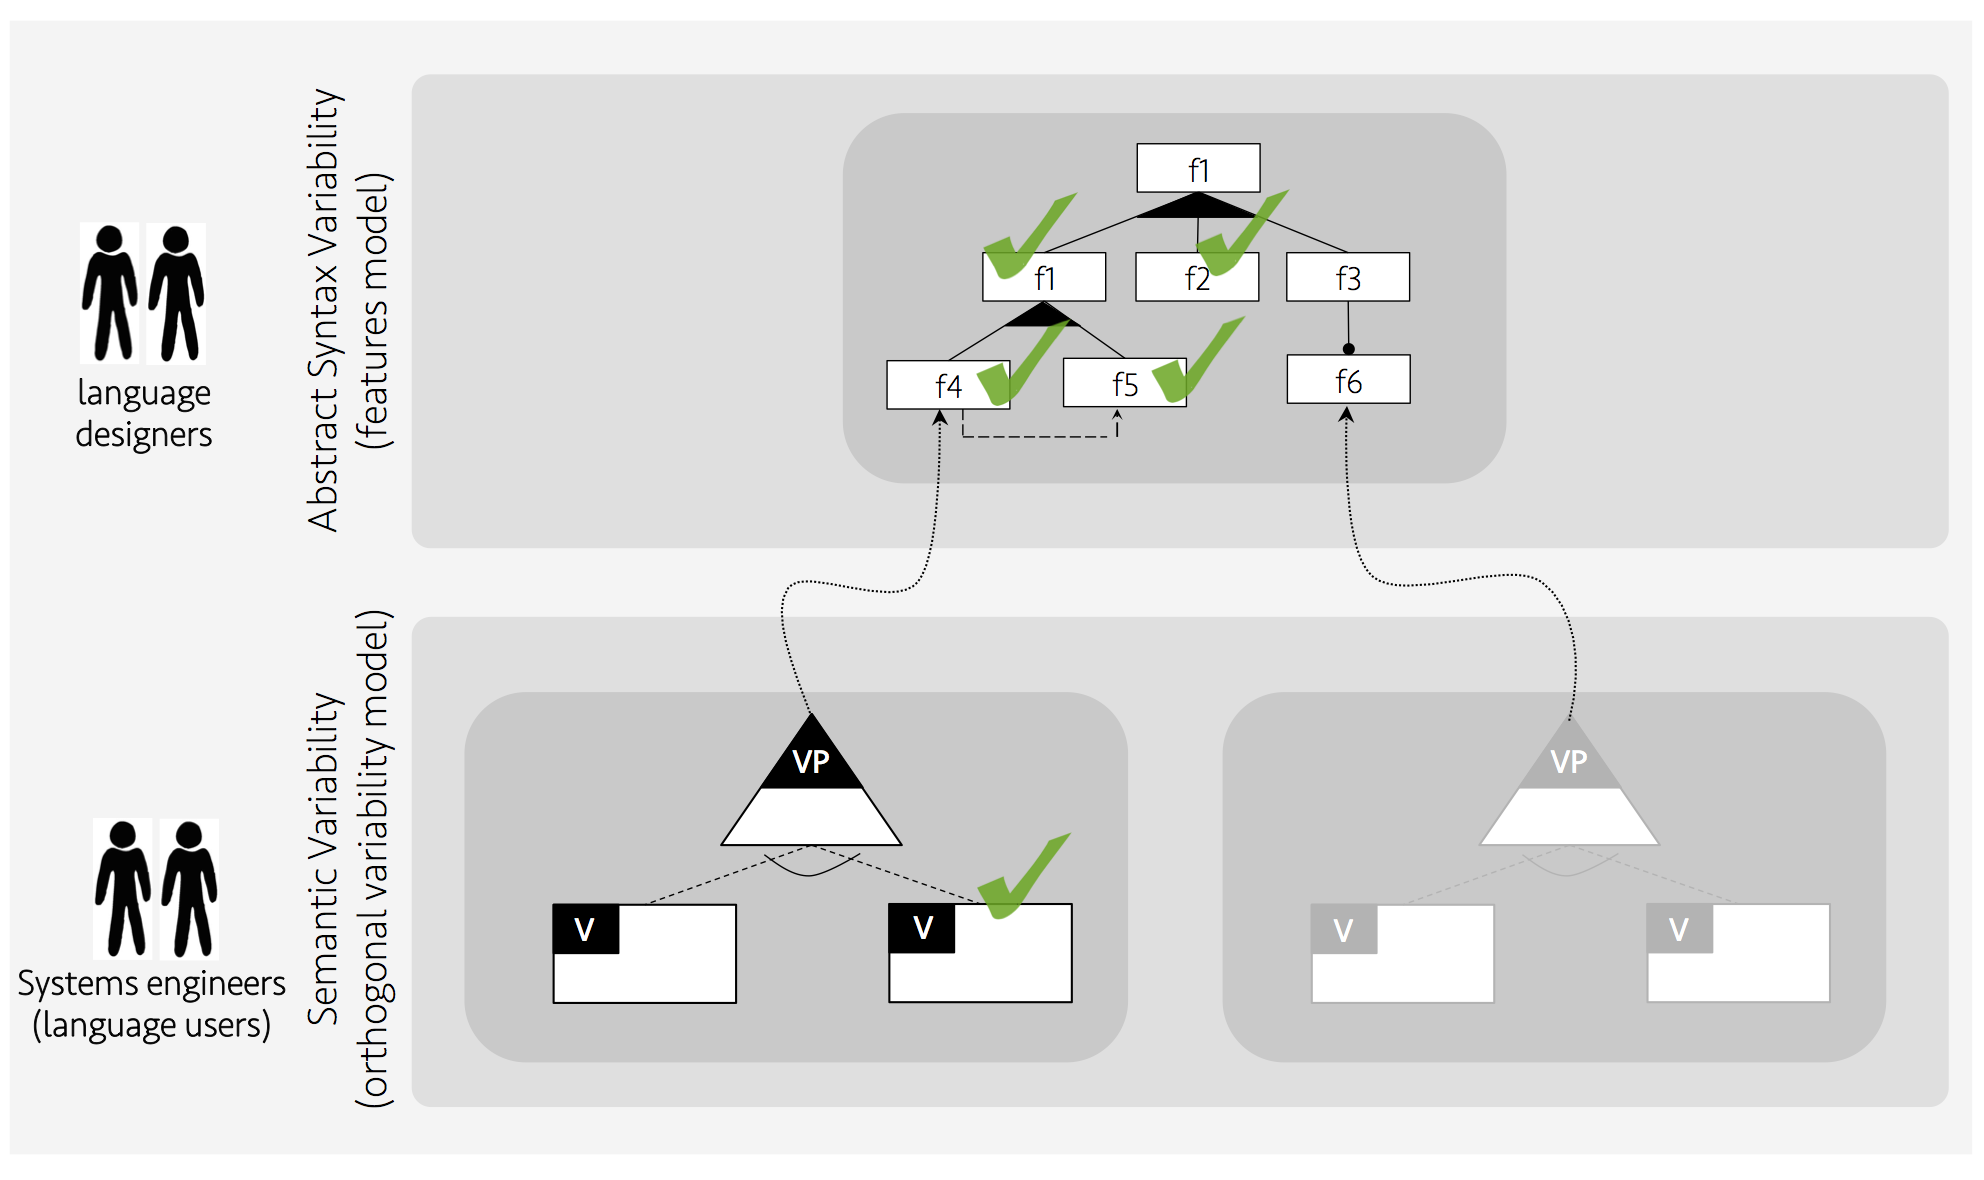
\includegraphics[width=1\linewidth]{images/languages-configuration-fig.png}
  \caption{Approach to support multi-staged configuration of language product lines}
  \label{fig:languages-configuration-modeling}
\end{figure}

\subsection{Language Modules Composition}

The final step of the language product line engineering process is the composition of the language modules corresponding to the configuration indicated in the variability models. This composition process starts by checking the compatibility between the required and provided interfaces of the involved modules. Then, the specification of the modules are merged to produce a complete DSL variant.  

\vspace{2mm}
\textbf{\textit{Compatibility checking.}} To establish a compatibility checking mechanism between provided and required interfaces, we need to conciliate two different (and potentially conflicting) issues. Firstly, such a compatibility checking must guarantee safe composition of the involved language modules. Hence, we need to verify that the functionality offered by the provided interface actually fulfills the needs of required interface. Secondly, there must be some place for substitutability. Hence, compatibility checking should offer certain flexibility that permits to perform composition despite some differences in their definitions. This is important because when language modules are development independently of each other, their interfaces and implementations not always match \cite{Gschwind:2012}.

To deal with the aforementioned issues, we propose an approach for compatibility checking which is at the same time strict enough to guarantee safe composition, and flexible enough to permit substitutability under certain conditions. We extract both required and provided interfaces in the form of \textit{model types} \cite{Steel:2007}. The model type corresponding to the required interface contains the required specification elements of a language module whereas the model type corresponding to the provided interface the model type contains its public specification elements \footnote{The relationship between a model type and a language module is called \textsl{\textbf{implements}} and it is introduced by Degueule et al. \cite{Degueule:2015a}.}. Then, we perform compatibility checking by checking the sub-typing relationship --introduced by Guy et al. \cite{Guy:2012}-- between the model types corresponding to the provided and the required interfaces. This relationship imposes certain constraints that guarantee safe composition while permitting some freedom degrees thus introducing some flexibility. %In particular, under this definition of sub-typing the most obvious manner to guarantee safe composition is to check two conditions: (1) all the needs expressed in the requiring model type are furnished in the providing model type (\textbf{total} sub-typing); and (2) the two model types have exactly the same shape (\textbf{isomorphic} sub-typing). However, this definition of sub-typing also provides two dimensions of flexibility: \textbf{partial} sub-typing and \textbf{non-isomorphic} sub-typing. 

%The main principle behind partial sub-typing is that not all the needs expressed in the required model type must be provided by the provided one. In that case, compatibility checking corresponds to verify that the sub-set of elements that match in the model types are compatible. Then, the result of the composition is a third language module with a resulting required interface that contains those needs that have not been satisfied by the providing language module. 

%As an example suppose a language module for finite state machines that needs not only constraints for expressing guards in the transitions, but also action scripting constructs to express the behavior of the states. In such a case, a constraint module will fulfill the first need but not the second one. Thanks to partial sub-typing, we can perform compatibility checking only on the constructs associated to the constraints and, if they are compatible, then compose those language modules. The result will be a language module having the constructs for state machines and constraints but that still needs action scripting constructs defined in its required interface.

%The principle behind isomorphic sub-typing is that the needs in the requiring interface are not always expressed exactly as the functionality offered by the providing module is expressed in the providing interface. For example, model type in Fig. \ref{fig:fig-req-example-fig} expresses the needs in terms of constraints of state machines through a class \textsl{Constraint} with an operation \textsl{eval()}. If we want to use OCL to satisfy these needs, then we will find that there is not a class constraint but \textsl{OclExpr}. Besides, the operational semantics might be implemented differently. In this case, we need an adapter that permit to find the correspondences among the elements of the model types. 

\vspace{2mm}
\textit{\textbf{Merging modules' specifications.}} The process of merging the specification of a set of language modules is performed in two phases. First, there is a matching process that identifies one-to-one matches between required and public elements from the required and provided interface respectively. This match can be identified automatically by comparing names and types of the elements (where applicable). However, the match can be also specified manually in the case of non-isomorphism.

Once the match is correctly established, the composition process continues with a merging algorithm that replaces virtual elements with public ones. When the process is finished, we re-calculate both provided and required interfaces. The provided interface of the composition is re-calculated as the sum of the public elements of the two modules under composition. In turn, the required interface of the composition is re-calculated as the difference of the required interface of the required module minus the provided interface of the providing module. 


% !TEX root = ../elsarticle-template.tex
%-------------------
\section{Case Study: The VaryMDE Project}
\label{sec:validation}

In this section, we introduce the VaryMDE project which is bilateral collaboration between INRIA and Thales Research \& Technology (TRT). The role of this project in the research presented in this article is two-fold. On one hand, it provides a set of research questions that motivate our work. Concretely, the research presented in this article represents an answer to some of the needs emerging in Thales in terms of language engineering. On the other hand, this project provides a realistic application scenario which we used as validation of the approach. In the reminder of this section, we present an overview of the project and we discuss the results of applying our approach in the scenario introduced by Thales.  

%INRIA' Diverse team worked togueter with Thales Research \& Technology (TRT) researchers towards targueting variability management issues at both the modeling level and the metamodeling level (i.e., design and implementation of software languages). Concretely, Thales researchers ended up having DSLs defined using three finite-state machines specifications and needed supoprt to avoid future costs. In the Section \label{sec:validation} we present more details about the used case.

 %To evaluate of our approach, we use a set of DSLs for state machines. Note that a simplified version have been used as running example along this paper (see Section \ref{sec:thedevelopmentscenario}). This scenario is inspired from the analysis of variability on languages for finite state machines provided by Crane et al. \cite{Crane:2007}, and it is composed of three different DSLs: UML state diagrams, Rhapsody, and Harel's state charts. As aforementioned, these DSLs have some commonalities since they are intended to express the same formalism. According to the development scenario we address in this paper, these commonalities will be materialized as clones in the DSL specifications. In this section, we summarize both commonalities and differences existing in the case study. Then, we apply our approach and we present the obtained results. To explain this scenario we try to follow as close as possible the guidelines provided by \cite{runeson-book} for the sake of clarity and organization. Note that we do not claim this to be a case study.

\subsection{Background to the research project}
Thales is a company whose business model turns around the construction of different types of systems that solve needs in diverse domains such as transport, aerospace, security, or defense. During the construction of these systems, Thales' engineers often appeal to the use of state machine languages to express behavior.

Despite the expressibility of state machines, the diversity of the systems built by Thales imposes an accidental complexity. Depending on the type of system under construction, there are different requirements on the way in which a state machine should be executed. Hence, there is certain semantic flexibility that state machine languages should offer to support the particularities of the systems unde construction. As a result, Thales engineers are intended to build not only the devices themselves but also to adapt the state machines formalisms. 

The typical development process to address the implementation of the formalisms for state machines is as follows: at the beginning, language designers build an initial DSL for state machines that fits the needs of one type of system. Then, they create new development branches when they adapt the first variant of the DSL to the needs of other types of systems. After some repetitions, language designers have a family of DSLs for state machines. Those DSLs have both syntax and semantic differences. 

\subsection{Design of the case study}

\textbf{Objectives.} One of the challenges of the VaryMDE project is to find out a way to facilitate the development process descrived above. As an answer of this challenge, we propose the use of reverse engineering techniques to create language product lines of DSLs for state machines from existing variants.

\vspace{2mm}
\textbf{Planning.} The case study was planned in three phases as shown in Fig. \ref{fig:planning}. In the first phase, the data set is prepared. Such a data set corresponds to the set of DSL variants that will be used to reverse engineer the language product line. This phase is iterative since we need to consider the feedback comming from the Thales' engineers. During the second phase, we execute our approach using the initial set of DSL variants. Finally, in the third phase we analyse the produced language product lines. 

\begin{figure}[h!]
	\centering
	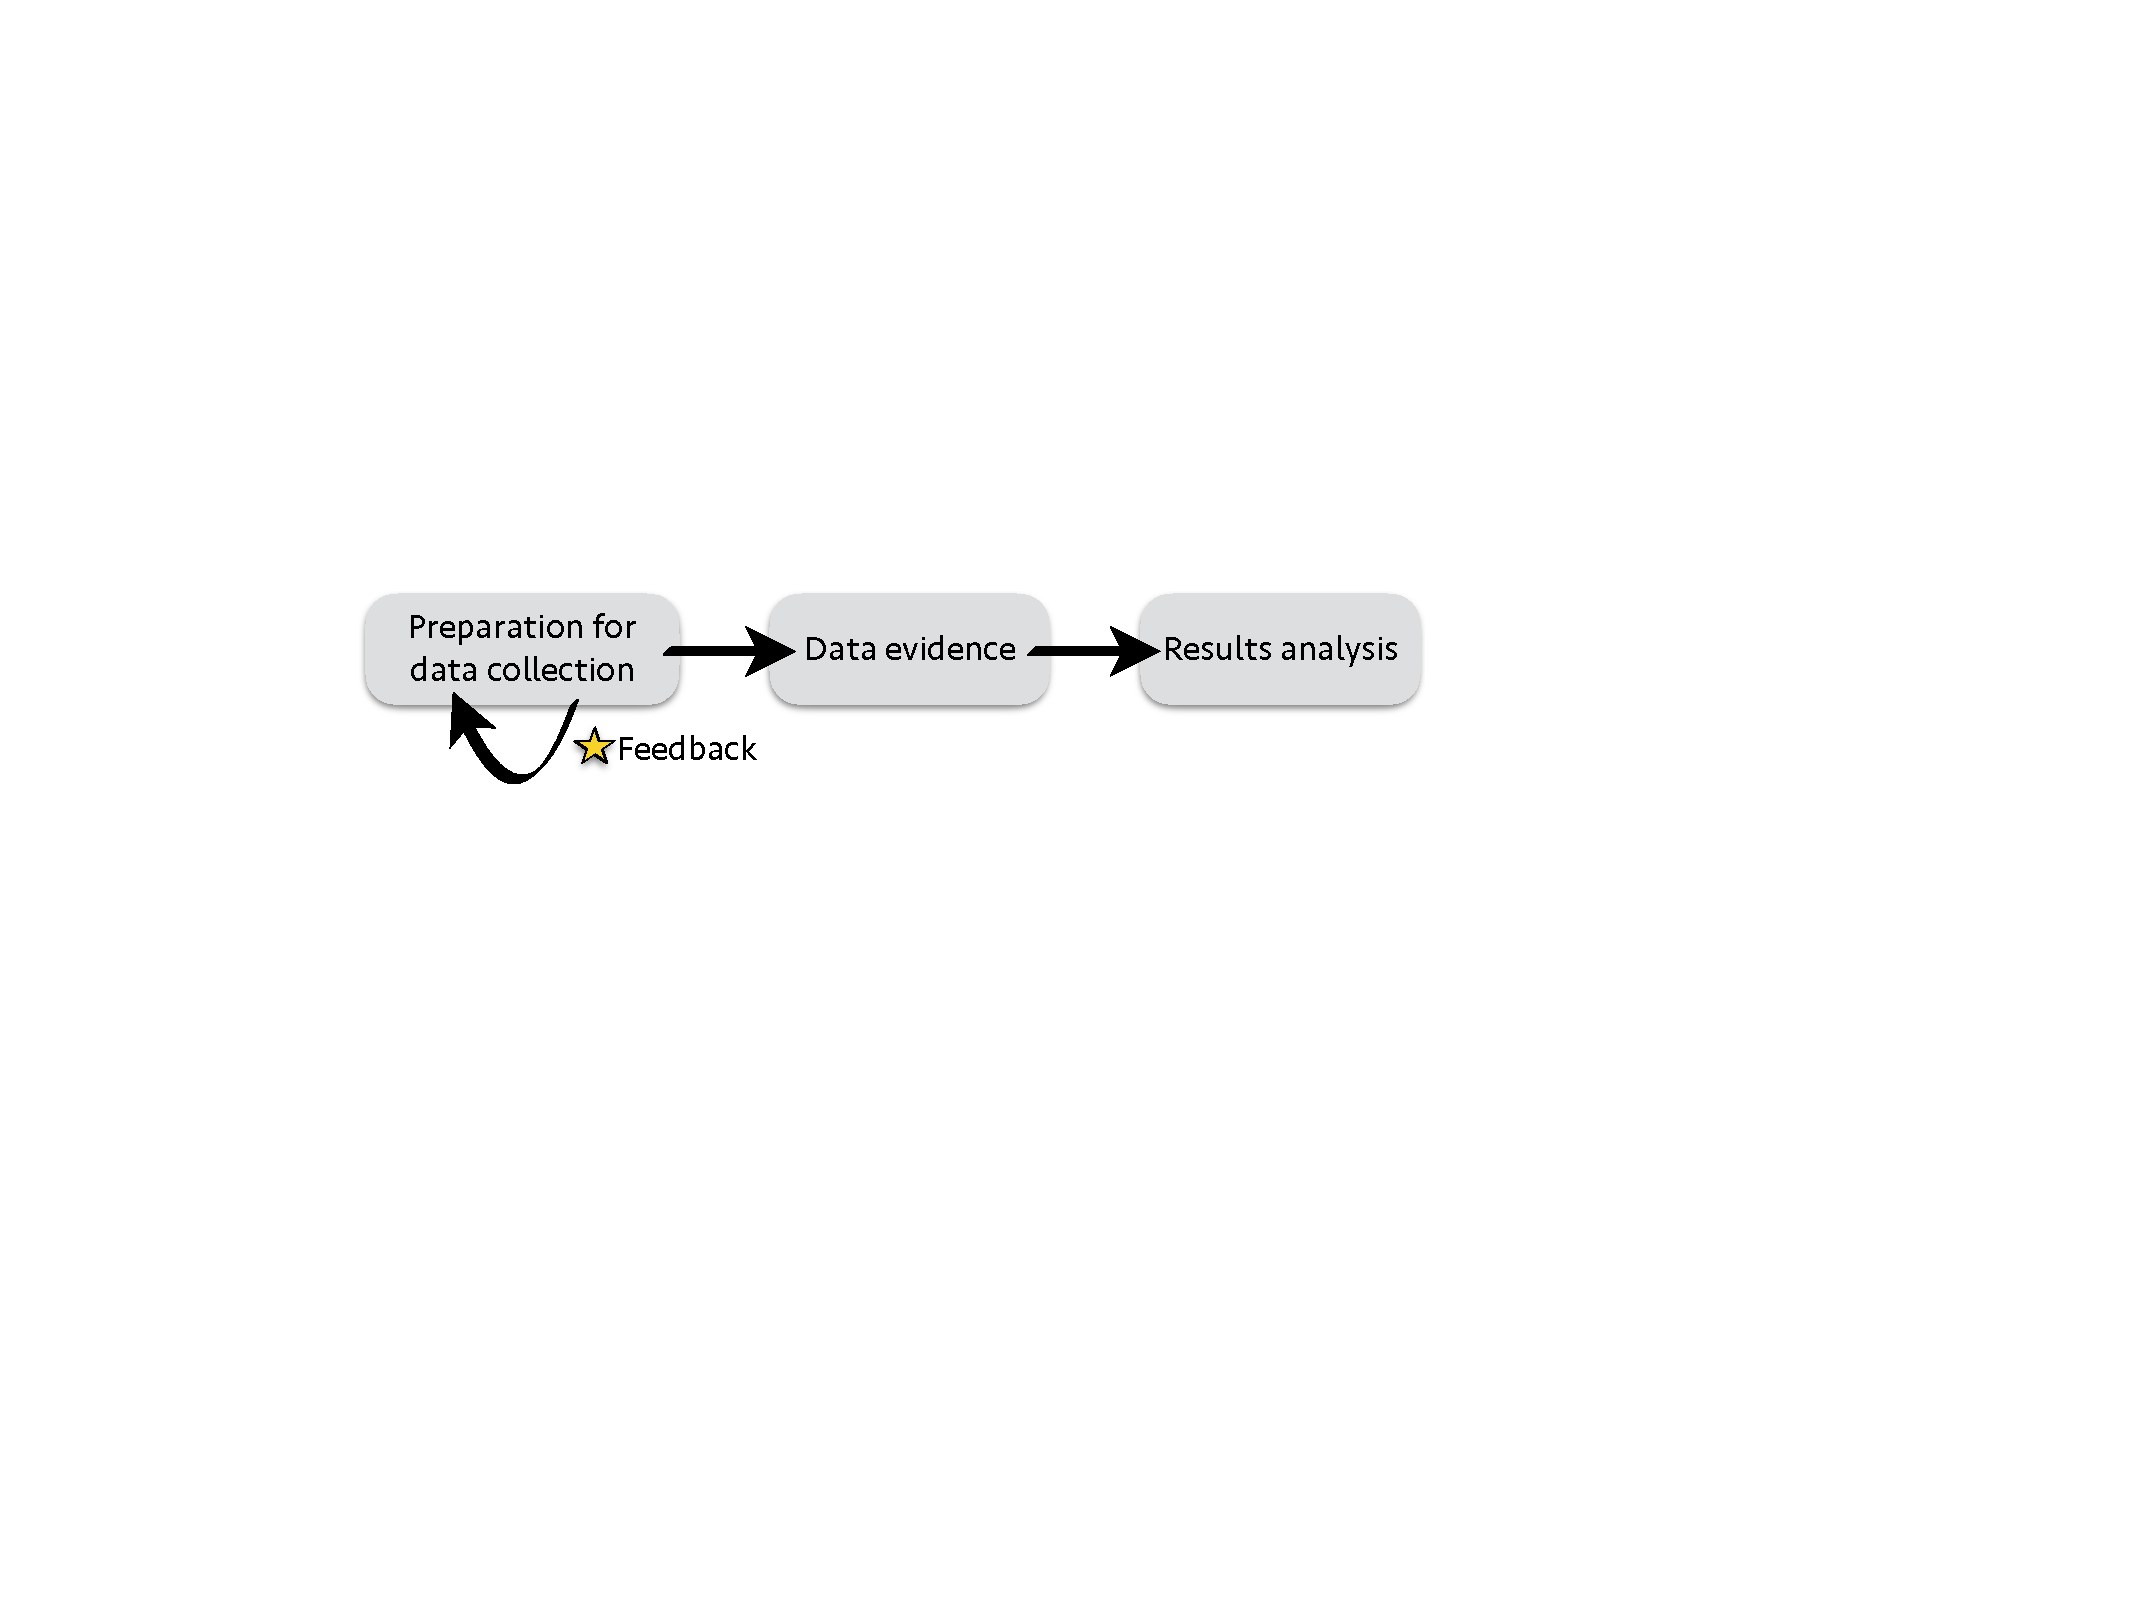
\includegraphics[width=1\linewidth]{images/planning-casestudy-fig.pdf}
	\caption{Planning of the case study}
	\label{fig:planning}
\end{figure}

\subsection{Preparation for data collection}

As aformentioned, the objective in this phase is to define the set of initial DSL variants that will be used to execute our approach. The most important limitation we found at this stage is that many of the implementations for state machine DSLs are built in different language workbenches and using diverse language meta-languages. Under these conditions, commonalities and particularities of DSLs are more difficult to detect.

To overcome such a limitation, we decided to implement the initial DSL variants in a unified language workbench and using the same meta-languages. Hence, the phase of preparation for data collection corresponds to a language development process where three different formalisms for state machiens were implemented: UML state machines, Rhapsody, and Harel statecharts. Those formalisms were selected because they have a complete documentation that allow to fully understand its semantics. The implementation of the formalisms was conducted on top of Melange \cite{Degueule:2015a} language workbench and it is available on a dedicated GitHub repository\footnote{GitHub repository: \url{https://github.com/damende/puzzle/tree/master/examples/state-machines}}. The description of commonalities and differences existing among the selected formalisms are well-studied by Crane et al and are described in Annexe A. 

\subsection{Collecting evidence}

Once we built the initial set of DSLs variants, we execute our approach and obtained a language product line for state machines. The results are summarized in Fig. \ref{fig:results-casestudy}. At the left of the figure we present the set of language modules we obtained as well as the language interfaces existing among them. Those modules group the language constructs according to the heuristic introduced in Section \ref{sec:reverseengineeringmodules} on breaking down intersections. At the right of the figure we show the corresponding variability models. Each feature of the feature models is associated to a given language module. In turn, the semantic variability points in the orthogonal model are associated to clusters of domain specific actions.

%Note that we marked different configurations in the figure to identify each of the corresponding DSLs. In addition, we calculated the number of possible configurations. We obtained that with this variability model, we can obtain XXX DSLs for state machines.

\begin{figure*}
	\centering
	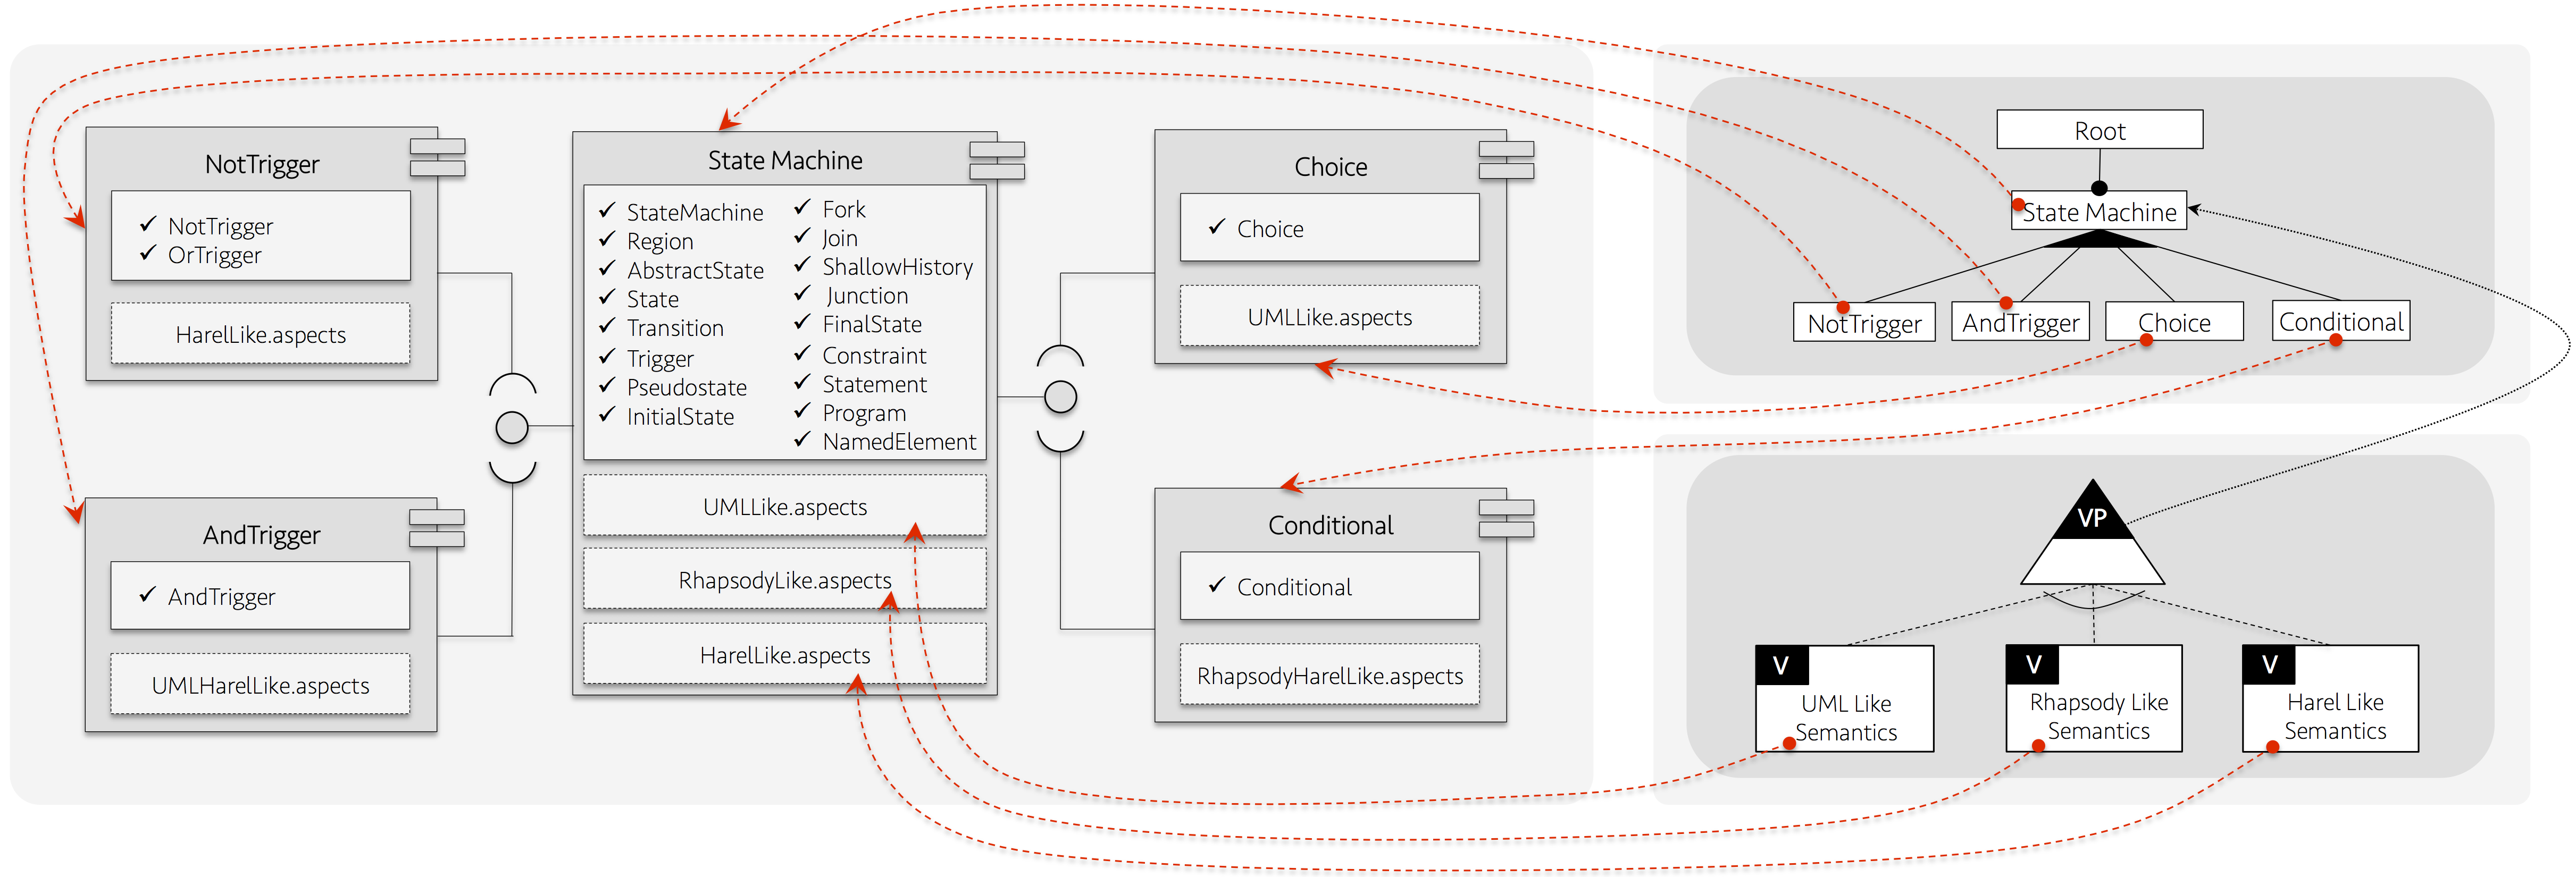
\includegraphics[width=1\linewidth]{images/results-casestudy.png}
	\caption{Language product line produced for the case study of the finite state machines. }
	\label{fig:results-casestudy}
\end{figure*}

\subsection{Analysis of collected data}

Let us now discuss the results of the case study. As expected, we obtained a language product product line from a set of DSL variants for finite state machines. But... Does this product line identify all the variation points and commonalities existing in the DSL variants? Are those variation points properly specified in the language modular design and variability models? Since we know these variation points and commonalities, we can check whether they are appear in the produced language product line. The results of this verification are presented in Table \ref{fig:validation-results}.

The results are promising in the case of abstract syntax variability. According to the Table \ref{fig:oracle}, the DSL variants share 17 constructs in common. Those constructs are properly factorized in a language module that we named StateMachine. This module is correctly identified during the recovering of the language modular design, and it is properly specified as a language module in terms of a metamodel enhance with domain specific actions and offering a provided interface. Besides, the particularities of the DSL variants are also well factorized. There is a module that contains the constructs NotTrigger and OrTrigger that belong only to the variant complying the Harel' statecharts specification. Besides, there are three additional modules that contain the constructs AndTrigger, Choice, and Conditional respectively. Using this modular design, we can re-compose any of the three initial DSL variants.

The situation is different for the case of semantic variability. Although our reverse-engineering strategy is able to identify that the domain specific actions are different in the three DSL variants, the level of granularity at which those variation points are detected is coarser than one might expect. At the beginning of this section, we described three semantic variation points and their possible interpretations i.e., events dispatching policy, execution order of transitions' effects, and priorities of conflicting transitions. Using the proposed technique, we can identify just one semantic variation point indicating that the language module called StateMachines contains three different clusters of domain specific actions, which is reflected in the orthogonal variability model.

This threat to validity of our technique can be explained by the fact that the analysis of commonalities and variability is conducted by means of static analysis. We can analyze the structure of the metamodels and the domain specific actions, but not their behavior at runtime. Hence, we cannot see how these differences impact the execution of the models. For example, we cannot infer that the differences among the domain specific actions in the StateMachine module impact the way in which conflicting priorities are managed. A next step in this research could be to use also dynamic analysis in the domain specific actions to better specify semantic variation points.

\begin{table}
\centering
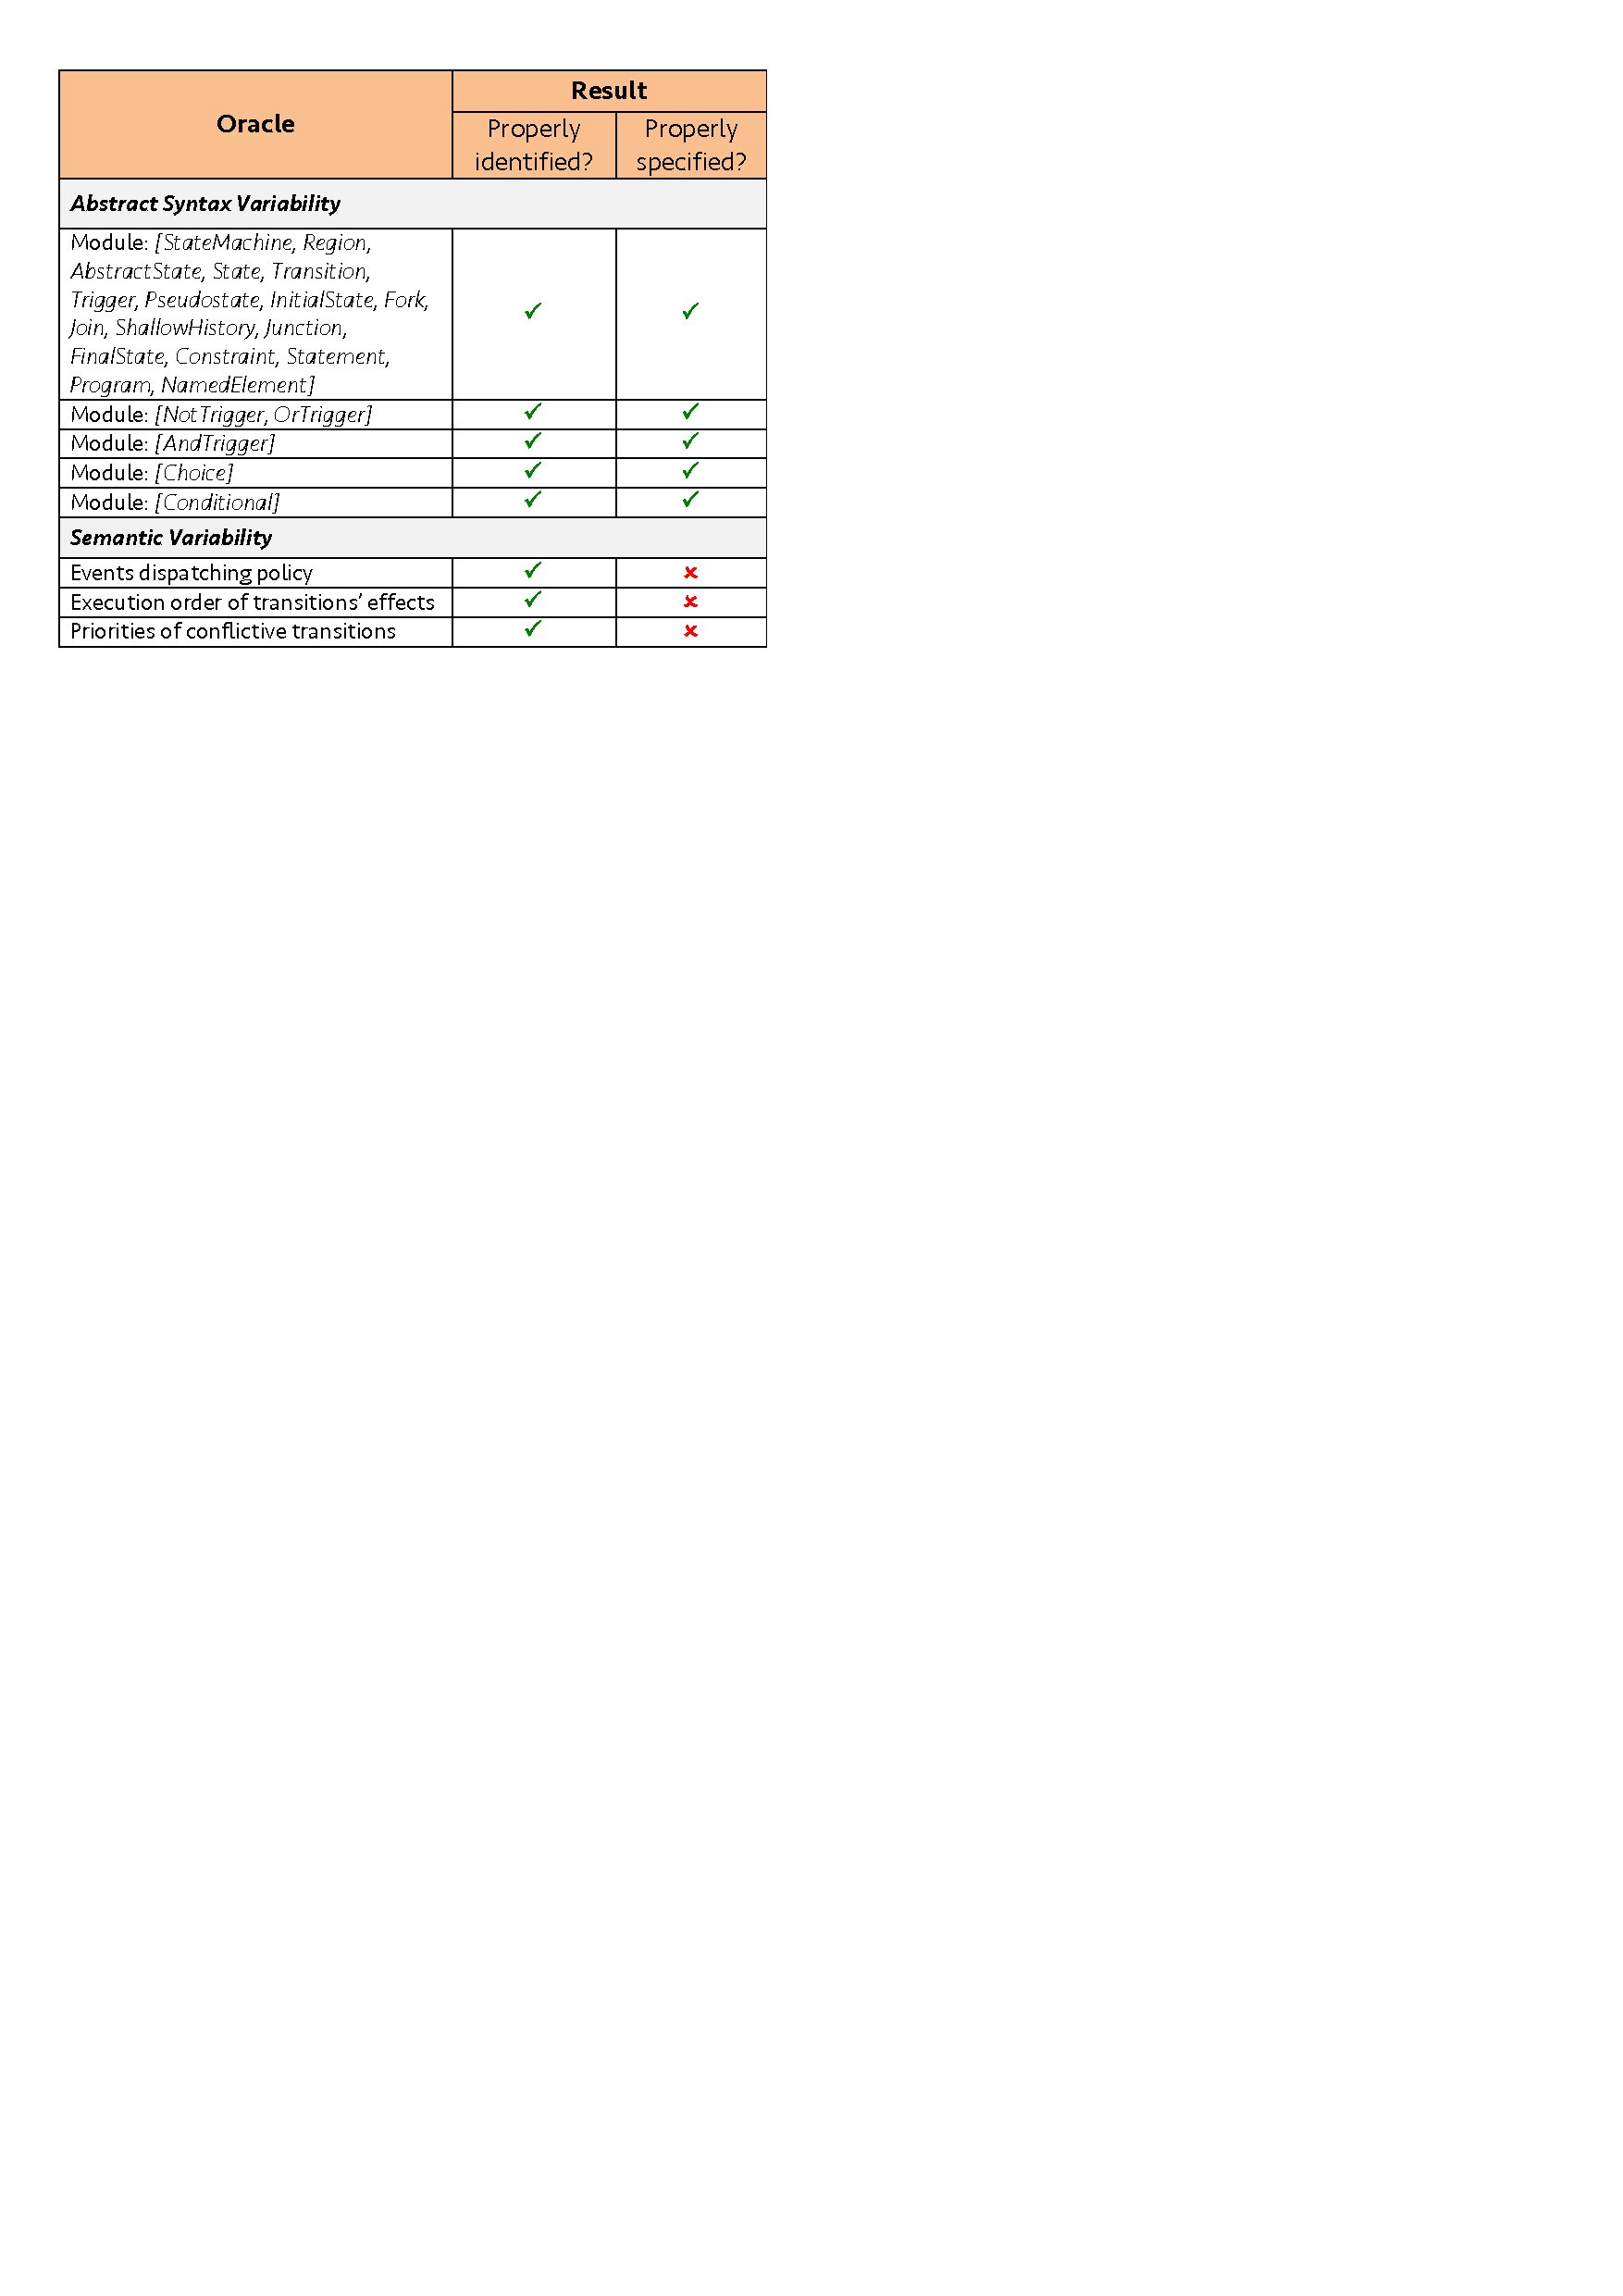
\includegraphics[width=1\linewidth]{images/validation-results}
\caption{Analysis of the results of the case study}
\label{fig:validation-results}
\end{table}

%\subsubsection{Units of Analyses}
%Three different formalims were considered i) UML; ii) Rhapsody, and; iii) Harel's statecharts. For each of take a look to two properties of them. First, the commonalities, this is the common parts to all the existing state machines formalisms. Second, the variabilities or the parts that differ between the different formalims.

%\paragraph{Methods, data collection and measures}
%The main source of information in this enquiry is the set of meetings that some of the authors had with the representative of the Thales side of the project. A total of \todo[inline]{XX} meetings were held. After the first one a set of software artifacts were provided for a detailed analysis as well as the requisites for each formalism.

%The data were collected in the following ways

%\begin{itemize}
%	\item Artifacts analysis, we received from Thales a set of models and metamodels depicting the diferent state machines that the thales group uses.
%	\item Interviews, we performed several meeting to ask for the aplications and plans for the metamodels and its variabilities and commonalities.
%\end{itemize}
%\section{Threads to validity}
\label{sec:limitations}
\section{Related Work}
\label{sec:relatedwork}

The idea of reverse engineering software product lines from product variants has been already studied in the literature. Besides, there are several approaches that address this issue for the case in which the product variants have been built using the clone-and-own approach \cite{LopezHerrejon:2015,Martinez:2015,Martinez:2015b}. Although the applicability of such idea to the specific case of language product lines is quite recent, there are some related work that we discuss in this section. 

\vspace{2mm}
\textbf{\textit{Recovering a language modular design.}} The first challenge during reverse engineering language of product lines is to recover a language modular design. Although this challenge has not received proper attention, we found an approach that proposes insightful advances in this direction \cite{Kuhn:2015}. In that work, the language modular design is achieved by defining one language module for each construct. That means that the reverse engineering process will result in a language product line containing as many features as constructs exist in the DSLs.

This approach permits to exploit the variability in the language product line since it provides a high level of granularity in the decomposition of language modules. Hence, language designers can make decisions with an important level of detail. However, the complexity of the product line might increase unnecessarily. From the point of view of language users, there are clusters of language constructs that always go together thus separation is not needed. For example, in our running on state machines, the concepts of \texttt{StateMachine}, \texttt{State}, and \texttt{Transition}, go always together since they correspond to a commonality of all the input DSLs. Separating these constructs in different features is not necessary in this case and this increases the complexity of the variability models. This can be a real issue if language designers decide to apply automatic analysis operations on those models.

Differently, in our approach we use the notion of specification clones and intersections in order to achieve a level of granularity that captures the variability existing in the DSL variants given in the input. This permits to identify those clusters of language constructs that go always together in the given variants. This decision simplifies the language product line in the sense that the amount of language modules is lower than in the approach by Kuhn et al., \cite{Kuhn:2015}. In doing so, we certainly reduce the possible variants that can be configured by the language product line. This issue can be considered as a threat to validity of our approach. 

\vspace{2mm}
\textbf{\textit{Synthesizing variability models.}} The synthesis of variability models has been largely studied in the literature. Some of those approaches have been adapted for the particular case of variability in the context of language product lines engineering. The approach presented in \cite{Vacchi:2014} proposes a search-based technique to find a features model that represents the variability existing in a set of language modules while optimizing an objective function. This approach uses an ontology that describes the domain concepts of the language product line. The second approach (presented in \cite{Kuhn:2015}) refines the former by removing the ontology. This improvement is motivated by the difficulty behind the construction of such ontology. Then, the authors propose to annotate the BNF-like grammar with certain information that is used to create a variability model. 

The aforementioned approaches support not only abstract syntax variability, but also concrete syntax and semantic variability. In the first case, the ontology can be used to identify all the existing syntactic and semantic variation points since it represents the domain from both the syntax and semantic point of view. In the second case, the annotations provide the expressiveness enough to address all these dimensions of the variability.  

There is, however, an important limitation in those approaches. Although at the modeling level, feature models have shown their capabilities to represent multi-dimensional variability and it has been validated for language product lines, there is not support for effectively reverse-engineering such multi-dimensional variability in the language product lines. Indeed, the solution provided by current approaches is to synthesize variability models where each feature capture both the abstract syntax of the language constructs and their semantics. Using this strategy, a language construct that has different semantics interpretations is represented as two language features. Those features have the same abstract syntax (a repeated definition of the specification) and their corresponding semantics. 

The problem with this strategy is that it couples abstract syntax variability with semantics variability, which limits multi-staged configuration. The scenario in which language designers configure only the abstract syntax, and final users configure their semantics is not supported since the configuration of the semantics depends also to configure a segment of the abstract syntax. 

We claim that, in order to facilitate multi-staged configuration, the abstract syntax variability should be defined separately from the semantic variability. The main contribution of our approach constitutes an answer to that claim. We use feature models to represent abstract syntax variability, and orthogonal variability models to represent semantics variability.  

\section{Discussion: Broadening the Spectrum}

The approach presented in this article is only useful when language designers follow the development scenario described in Section \ref{sec:thedevelopmentscenario} while using the technological space mentioned in Section \ref{sec:technologicalscope}. Along this paper we show how we can reduce maintenance costs and exploit variability if those conditions are fulfilled. In this section we open the broaden by discussing potential directions to support more diverse scenarios. 

\vspace{2mm}
\textit{Thinking outside the clone-and-own approach.} An important constraint of our approach is that it is scoped to DSLs that have been built through the clone-and-own approach. This fact permit to assume the existence of specification clones which is the backbone of our strategy for reverse engineering language modules. But... what if we have DSLs that are not necessarily built in those conditions? Suppose for example that we have as input a set of DSLs that share certain commonalities but that have been developed in different development teams. In that case, the probability of finding specification scenarios is quite reduced, and our approach will not be useful. How our strategies can be extended to deal with such a scenario?

The answer to that question relies on the definition of more complex comparison operators. As we deeply explain in Section \ref{sec:reverse-engineering}, the very first step of our reverse engineering strategy is to perform a static analysis of the given DSLs and apply two comparison in order to specify specification clones. If what we want is to find commonalities that are not necessarily materialized in specification clones but in "equivalent functionality", then we need to enhance the comparison operators in order to detect such as equivalences. 

Note the complexity behind the notion of "equivalent functionality". In the case of abstract syntax, two meta-classes might provide equivalent functionality by defining different language constructs e.g., using different names for the specification elements and even different relationships among them. In the case of the semantics, two different domain specific actions might provide equivalent functionality through different programs. We claim that further research is needed to establish this notion of equivalence thus supporting more diverse development scenarios. 

%\vspace{2mm}
%\textit{Thinking outside metamodels and domain specific actions.} Another issue to consider is the comparison of the DSLs specifications. In our case, we propose a comparison operator that is quite strict in the sense that it validates that all the specification elements are the same. This guarantees that the is actually copy paste and permits to do the division in a safe way. However, we can loose some reuse opportunities. For example, .... We claim that there is room for better developing the comparison operators. We can for example, consider issues such as .. subtyping, or even. 

%At the implementation level we provide an interface that facilitates this process. 

%\textit{On the purpose of the modular design} The reverse engineering process is guided by a clear purpose. In our case, the purpose is to reduce the maintenance costs of the DSLs. This is evidenced in the breaking down strategy which is mainly focused on removing the specification clones. A direct consequence of this is that we are able to support the variation points existing in the given set of DSLs. For example, we know that the is one language supporting AND and OR triggers. However, our approach is limited to the variation points existing in the input DSLs. If for example, we want to create a new DSL that contains only ANDTrigger, the produced language product line will not permit that. Indeed, we consider that there is room for other strategies more intended to exploit the variability. For example, in the approach presented in X the division is performed at the level of the language constructs. Then, each feature represents one construct. The limitation of this approach, however, is that the variability models might become too large and the configuration process might be tedious. Other solution can be the support for human intervention during the breaking down process. Another solution might be the optimization of some well-designed principles. Indeed, we have some preliminary experiments by using meta-heuristics to optimize high-cohesion and low-coupling. The partial results are promising but in that case the development scenarios are quite diverse. 

%It is wort mentioning that at implementation level of our approach is conceived in such a way that the modularization strategy can be easily replaced. Indeed, we provide the interface IBreaker that supposes the method break. It receives a set of DSLs and it returns the set of language modules. In doing so, we facilitate the experimentation with new strategies that can be more appropriated to a particular context. 


\section{Conclusion}
\label{sec:conclusions}

In this article we presented an approach to support the construction of bottom-up language product lines. Our approach consists of a reverse-engineering process that allows to automatically produce a language product line from a set of DSL variants. Such reverse-engineering process starts by recovering a language modular design, and then produces variability models that permit configuration of new variants. We validate our approach in a project with industrial partners on different DSL variants to express finite state machines. 


\section*{Acknowledgments}
This work is supported by the ANR INS Project GEMOC (ANR-12-INSE-0011); the bilateral collaboration VaryMDE between Inria and Thales; the bilateral collaboration FPML between Inria and DGA; and the European Union within the FP7 Marie Curie Initial Training Network “RELATE" under grant agreement number 264840. 
\section*{References}

\bibliography{mybibfile}

\end{document}
